\documentclass[12pt]{article}
\usepackage[T1]{fontenc}
\usepackage[polish]{babel}
\usepackage[utf8]{inputenc}
\usepackage{lmodern}
\selectlanguage{polish}
\usepackage{graphicx}
\usepackage{mathtools}
\usepackage{spverbatim}
\usepackage{float}
\linespread{1.25}
\usepackage{array}
\graphicspath{{/home/franek/Documents/magisterka/images/}}

\title{Praca magisterska}
\author{Franciszek Słupski}
\date{Brak}

\begin{document}

\maketitle

\tableofcontents
\section{Wstęp}

\subsection{Testowa baza danych}
Aby przedstawić techniki optymalizacji zawarte w pracy na rzeczywistych przykładach, wykorzystałem bazę danych udostępnioną przez portal stackoverflow.com. Baza zawiera w granicach 50 Gb danych zebranych w latach 2008-2013. Archiwum po zaimportowaniu do serwera MySQL nie zawiera klucz głównych, kluczy obcych, indeksów.
Początkowy schemat bazy danych jest przedstawiony na rysunku 1.
\begin{figure}
    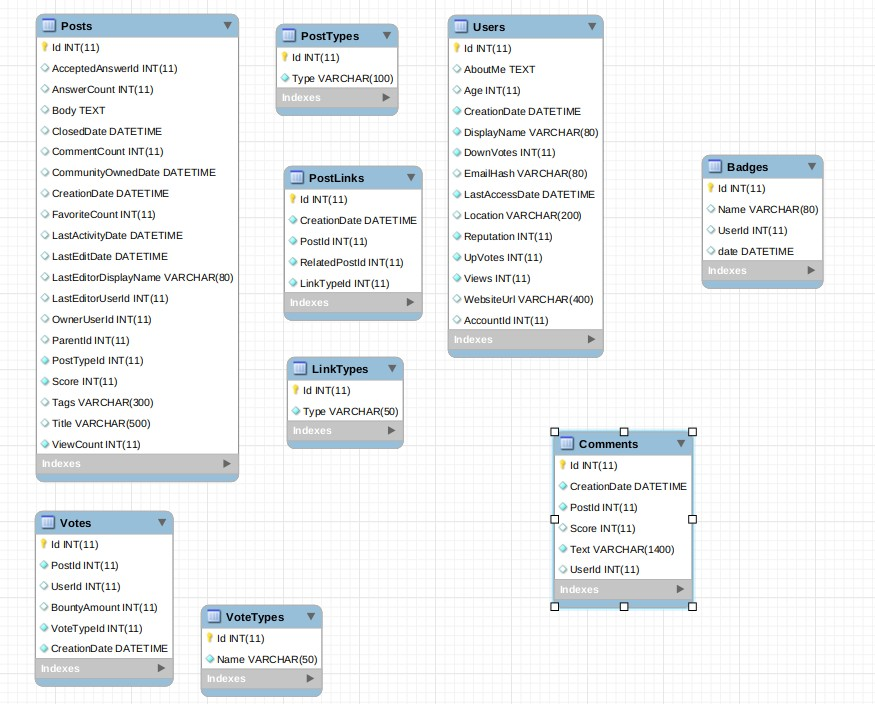
\includegraphics[scale =0.5]{schemat-baza-stackoverflow.jpg} 
    \caption{Schemat bazy danych stackoverflow}
\end{figure}

\subsection{Porównywanie zapytań}
W rozdziale zostanie przedstawione działanie polecenia EXPLAIN. Polecenie to umożliwia uzyskanie informacji o planie wykonania zapytania. Jest podstawowym sposobem określenia, w jaki sposób MySQL wykonuje zapytania. Analiza wyników EXPLAIN jest zdecydowanie bardziej użyteczna od mierzenia czasów zapytań. Na czas wykonania zapytania mogą mieć wpływ zewnętrzne czynniki, które wprowadzą nas w błąd podczas badania wydajności danego zapytania. Pierwszym z nich jest cache zapytań. Przeprowadzając testy zapytania przy włączonym buforze zapytań, może zdarzyć się, że rezultat zapytania zostanie zwrócony z tego właśnie bufora. Doprowadzi to do sytuacji, kiedy nawet najbardziej niewydajne zapytania będą zwracane w ułamek sekundy.  Problem ze zwracaniem wyników z bufora zapytań możemy rozwiązać poprzez wyłączenie bufora zapytań lub dodanie modyfikatora SQL\textunderscore NO\textunderscore CACHE do zapytań. Drugim czynnikiem zaburzającym mierzenie czasów wykonania zapytań jest bufor MySQL. MySQL stara się przechowywać w pamięci często używane dane, dla przykładu indeksy. Jeżeli wykonujemy zapytanie dla tabeli, której indeks nie znajduje się w pamięci. Serwer pobiera indeks z dysku, co trwa. Następnie poprawiamy zapytanie w celu poprawienia wydajności i wykonujemy, aby sprawdzić, czy nasze działanie poprawiło wydajność. Tym razem cały indeks znajduje się w pamięci i zapytanie wykonuje się wielokrotnie szybciej. Mierząc jedynie czasy wykonania obu zapytań, możemy dojść do fałszywego wniosku, że drugie zapytanie jest wydajniejsze, nawet jeżeli w rzeczywistości nasze działanie doprowadziło do pogorszenia wydajności zapytania. W takim przypadku dobrym rozwiązaniem wydaje się kilkukrotne mierzenie czasów, obliczenie średniej i na tej podstawie porównywanie wyników. Dodatkowo nasz serwer rzadko kiedy jest całkowicie odcięty od świata. Bardzo często będziemy testować wydajność zapytań na tabelach, które są w równocześnie modyfikowane w tle. Przykładowo jeżeli testujemy zapytanie na tabeli, na której równocześnie wykonywane są operacje zapisu, czasy wykonania naszego zapytania nie będą miarodajne. Dodatkowo na czasy wykonywania zapytań wpływ może mieć aktualne obciążenie serwera, co nie ułatwia pracy przy porównywaniu wyników. Jak widzimy aby skutecznie porównywać wydajność zapytań nie powinniśmy opierać się jedynie na czasie ich wykonania.
\subsection{Polecenie EXPLAIN}
Polecenie EXPLAIN będzie jedną z głównych metod porównywania wydajności zapytań stosowaną w tej pracy, dlatego w tym podroździale przedstawie podstawy stosowania tego polecenia. Funkcja EXPLAIN to główny sposób określania, jaki sposób wykonania zapytania wybrany na etapie jego optymalizacji przez optymalizator MySQL.

Aby użyć polecenia EXPLAIN, wystarczy poprzedzić słowa kluczowe takie jak SELECT,INSERT,UPDATE,DELETE poleceniem EXPLAIN. Spowoduje to, że zamiast wykonania zapytania, sewer zwróci informacje o planie wykonania. Rezultat polecenia EXPLAIN zawiera po jednym rekordzie dla każdej tabeli użytej w zapytaniu. Kolejność wierszy w wyniku zapytania odpowiada kolejności, w jakiej MySQL będzie wykonywał zapytania.  Pierwszym zapytaniem wykonanym przez MySQL będzie zapytanie z ostatniego wiersza.

\subsubsection{Wyniki polecenia EXPLAIN}
Żeby zademonstrować wyniki polecenia EXPLAIN na rzeczywistych przykładach wykonałem kilka zapytań EXPLAIN na bazie StackOverflow. Dla porządku uznajmy, że zapytania są ponumerowane względem kolejności ich występowania w rozdziale.
\begin{spverbatim}
	SELECT u.DisplayName, c.CreationDate, c.`Text` FROM  Comments c LEFT JOIN Users u ON c.UserId = u.Id WHERE c.PostId = 875;
\end{spverbatim}
\begin{figure}[H]
	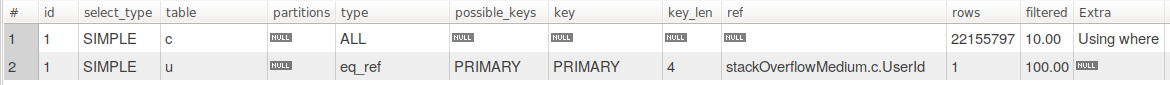
\includegraphics[scale =0.4]{explain7.png} 
	\caption{Przykład 1}
\end{figure}
\begin{spverbatim}
	SELECT p.Body FROM Posts p WHERE p.Id = 875 UNION
	SELECT c.`Text` FROM Comments c WHERE c.PostID = 875;
\end{spverbatim}
\begin{figure}[H]
	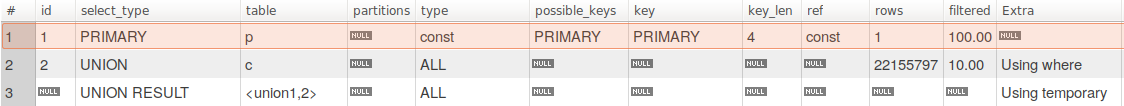
\includegraphics[scale =0.4]{explain8.png} 
	\caption{Przykład 2}
\end{figure}
\begin{spverbatim}
	SELECT * FROM Comments WHERE UserId = (SELECT id FROM Users WHERE DisplayName = 'Jarrod Dixon');
\end{spverbatim}
\begin{figure}[H]
	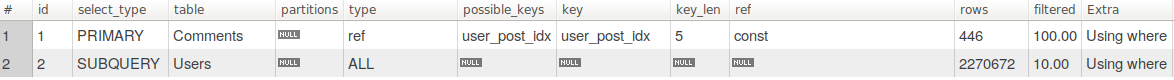
\includegraphics[scale =0.4]{explain9.png} 
	\caption{Przykład 3}
\end{figure}
\begin{spverbatim}
	SELECT * FROM Comments WHERE UserID in (SELECT UserId FROM Posts GROUP BY UserId HAVING COUNT(*) > 10);
\end{spverbatim}
\begin{figure}[H]
	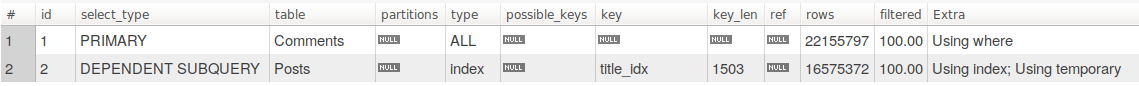
\includegraphics[scale =0.4]{explain9a.png} 
	\caption{Przykład 4}
\end{figure}
\begin{spverbatim}
	SELECT * FROM Comments WHERE UserID in (SELECT UserId FROM Posts GROUP BY UserId HAVING COUNT(*) > 10);
\end{spverbatim}
\begin{figure}[H]
	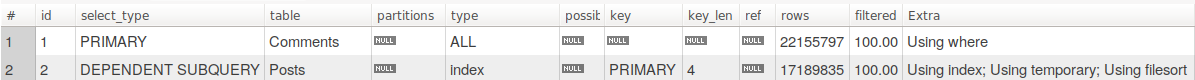
\includegraphics[scale =0.4]{explain10.png} 
	\caption{Przykład 5}
\end{figure}
\begin{spverbatim}
	SELECT * FROM Posts  WHERE OwnerUserId IN (SELECT id FROM Users WHERE Reputation>1000 UNION SELECT UserId FROM Comments WHERE Score >10)
\end{spverbatim}
\begin{figure}[H]
	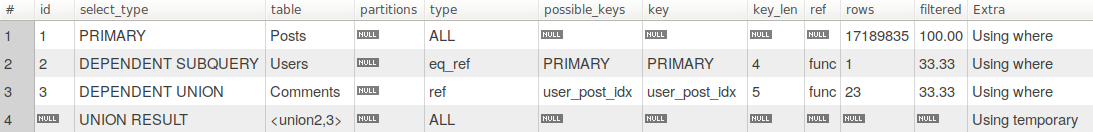
\includegraphics[scale =0.4]{explain11.png} 
	\caption{Przykład 6}
\end{figure}
\begin{spverbatim}
	SELECT * FROM Comments WHERE UserId = (SELECT @var1 FROM Users WHERE DisplayName = 'Jarrod Dixon');
\end{spverbatim}
\begin{figure}[H]
	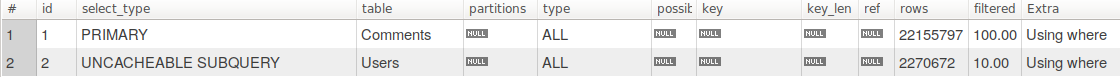
\includegraphics[scale =0.4]{explain12.png} 
	\caption{Przykład 7}
\end{figure}
\begin{spverbatim}
SELECT * FROM Comments LIMIT 10;
\end{spverbatim}
\begin{figure}[H]
	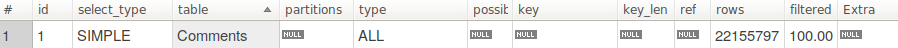
\includegraphics[scale =0.4]{explain13.png} 
	\caption{Przykład 8}
\end{figure}

\paragraph{Kolumna \#}
Wartości w kolumnie \# określają w jakiej kolejności MySQL będzie odczytywał tebele. Jako pierwsza odczytywana jest tabela z najmniejszą wartością.

\paragraph{Kolumna ID}\leavevmode\\
Kolumna id zawiera numer zapytania, którego dotyczy. W przypadku zapytań z podzapytaniami, podzapytania w dyrektywie FROM oraz zapytań z słowem kluczowym JOIN podzapytania numerowane są najczęściej względem ich występowania w zapytaniu. Kolumna ID może przyjąć również wartość NULL, w przypadku polecenia UNION (przykład 2).

\paragraph{Kolumna select\textunderscore type}\leavevmode\\
Kolumna select\textunderscore type pokazuje, czy rekord jest prostym, czy złożonym zapytaniem SELECT. 
Wartość \textbf{SIMPLE} oznacza, że zapytanie nie zawiera podzapytań, oraz nie używa klauzuli UNION.

Jeżeli natomiast zapytanie zawiera podzapytania lub wykorzystuje klauzulę UNION, to rekord dla kolumny select\textunderscore type przyjmie wartość \textbf{PRIMARY} (przykład 2). Jeżeli rekord dotyczy podzapytania oznaczonego jako PRIMARY, to będzie oznaczony jako \textbf{SUBQUERY} (przykład 3). Jako \textbf{UNION} zostaną oznaczone zapytania, które są drugim i kolejnym zapytaniem w klauzuli UNION. Pierwsze zapytanie zostanie oznaczone tak samo, jakby było wykonywane jako zwykłe zapytanie SELECT (przykład 2). \textbf{DERIVED} oznacza, że zapytanie jest umieszczone jako podzapytanie w klauzuli FROM, jest wykonywane rekurencyjnie i wyniki są umieszczane w tabeli tymczasowej. Wartość \textbf{UNION RESULT} oznacza wiersz, jako polecenie SELECT użyte do pobrania wyników z tabeli tymczasowej użytej przy poleceniu UNION (przykład 2). Jeśli polecenie SELECT zależy od danych znajdujących się w podzapytaniu lub znajdujących się w wyniki klazuli UNION, to zostanie oznaczone odpowiednio jako \textbf{DEPENDENT SUBQUERY} (przykład 5) lub \textbf{DEPENDENT UNION} (Przykład 6). Dodatkowo w przypadku, jeżeli wynik zwracany jest z \textit{zmaterializowanego widoku (eng. materialized view)}, zapytanie zostanie oznaczone jako \textbf{MATERIALIZED}. W przykładzie 7, który jest oczywiście nonsensowny, ale dobrze obrazuje sytuację, kiedy jako select\textunderscore type otrzymamy wartość \textbf{UNCACHABLE\textunderscore SUBQUERY}, która oznacza, że coś w podzapytaniu uniemożliwiło jego buforowanie. Analogiczną sytuację mamy, jeżeli wiersz zostanie oznaczony jako \textbf{UNCACHABLE\textunderscore UNION}, ale w tym przypadku niemożliwe jest oczywiście buforowanie wyników polecenia UNION.

\paragraph{Kolumna table}\leavevmode\\
Kolumna \textit{table} w większości przypadków zawiera nazwę tabeli lub jej alias, do której odnosi się dany wiersz wyniku polecenia \textit{EXPLAIN}. W przypadku gdy zapytanie dotyczy tabel tymczasowych możemy zobaczyć np. table: <union1,2> (przykład 2), co oznacza, że zapytanie dotyczy tabeli tymczasowej stworzonej na podstawie polecenia \textit{UNION} na tabelach z wierszy o id 1 oraz 2.
Odczytując kolejno wartości kolumny \textit{table} możemy dowiedzieć się, w jakiej kolejności optymalizator MySQL zdecydował się ułożyć zapytania. 

\paragraph{Kolumna Type}\leavevmode\\
Kolumna \textit{Type} informuje o tym, w jaki sposób MySQL będzie przetwarzał wiersze w tabeli. Poniżej przedstawiono najważniejsze metody dostępu do danych, w kolejności od najgorszej do najlepszej.

\subparagraph{ALL}\leavevmode\\
Wartość \textit{ALL} informuje o tym, że serwer musi przeskanować całą tabelę w celu odnalezienia rekordów. Istnieją jednak wyjątki takie, jak w przykładzie 8, w którym polecenie \textit{EXPLAIN} pokazuje, że będzie wykonywany pełny skan tabeli, a w rzeczywistości dzięki użyciu polecenia \textit{LIMIT} zapytanie będzie wymagało jedynie 10 rekordów.

\subparagraph{index}\leavevmode\\
MySQL skanuje wszystkie wiersze w tabeli, ale może wykonać to w porządku w jakim jest przechowywane w indeksie, dzięki czemu unika sortowania. Największą wadą jest jednak nadal konieczność odczytu całej tabeli. Co więcej, dane z dysku pobierane są z adresów, których kolejność wynika z użytego indeksu. Adresy te nie muszą zajmować na dysku ciągłych obszarów, a to oznacza, że czas odczytu danych może znacznie wydłużyć się. Jeżeli w kolumnie \textit{extra} jest dodatkowo zawarta informacja ''Using Index'' oznacza to, ze MySQL wykorzystuje indeks pokrywający (opisany w dalszej części pracy) i nie wymaga odczytywania innych danych z dysku – do wykonania zapytania wystarczają dane umieszczone w indeksie.

\subparagraph{range}\leavevmode\\
Wartość \textit{range} oznacza ograniczone skanowanie zakresu. Takie skanowanie rozpoczyna się od pewnego miejsca indeksu, dzięki czemu nie musimy przechodzić przez cały indeks. Skanowanie indeksu powodują zapytania zawierające klauzulę \textit{BETWEEN} lub \textit{WHERE} z < lub >. Wady są takie same jak przy rodzaju \textit{index}

\subparagraph{index\textunderscore subquery}\leavevmode\\
TODO przyklad
\subparagraph{unique\textunderscore subquery}\leavevmode\\
TODO przyklad
\subparagraph{index merge}\leavevmode\\
TODO przyklad
\subparagraph{fulltext}\leavevmode\\
TODO przyklad

\subparagraph{ref}\leavevmode\\
Jest to wyszukiwanie, w którym MySQL musi przeszukać jedynie indeks w celu znalezienia rekordu opowiadającego pojedynczej wartości.
Przykładem takiego zapytania może być wyszukiwanie numerów postów danego użytkownika w tabeli \textit{Comments} zawierającej indeks typu \textit{BTREE} na kolumnach \textit{UserId} oraz \textit{PostId}.

\begin{spverbatim}
	SELECT PostId FROM Comments WHERE UserId = 10;
\end{spverbatim}
Dodatkowo odmianą dostępu \textit{ref} jest dostępd \textit{ref\textunderscore or\textunderscore null}, który oznacza, że wymagany jest dodatkowy dostęp w celu sprawdzenia wartości NULL.


\subparagraph{eq\textunderscore ref}\leavevmode\\

Jest to najlepsza możliwa forma złączenia. Oznacza, że z tabeli odczytywany jest tylko jeden wiersz dla każdej kombinacji wierszy z poprzednich tabel. Z tego rodzaju złączeniem mamy do czynienia, jeżeli wszystkie kolumny używane do złączenia są kluczem głównym lub indeksem ''NOT NULL UNIQUE''. Przykładem takiego zapytania jest złączenie wszystkich komentarzy z postami bazując na kluczu głównym Id z tabeli Posts. 

\begin{spverbatim}
	SELECT * FROM Comments c JOIN Posts p ON c.PostId = p.id;
\end{spverbatim}

\subparagraph{const}\leavevmode\\
Przeważnie występuje w przypadku użycia w klauzuli WHERE wartości z indeksu głównego. Wtedy wystarczy jednokrotne przeszukanie indeksu, a na znalezionym liściu indeksu dostępne są już wszystkie dane z wiersza tabeli. Dla przykładu w bazie StackOverflow może to być zapytanie pobierające komentarz bazując na Id.
\begin{spverbatim}
	EXPLAIN SELECT * FROM Comments WHERE id = 93;
\end{spverbatim}

\subparagraph{NULL}\leavevmode\\
Oznacza, że serwer nie wymaga skanowania całej tabeli lub indeksu i może zwrócić wartość już podczas fazy optymalizacji. Przykładem takiego zapytania może być zwrócenie minimalnej wartości z indeksu tabeli.

\begin{spverbatim}
	SELECT MIN(UserId) FROM Comments;
	#Tabela Comments zawiera indeks BTREE na kolumnie UserID
\end{spverbatim}

\paragraph{Kolumna Possible\textunderscore keys}\leavevmode\\

Komulna possible\textunderscore keys zawiera listę indeksów, które optymalizator brał pod uwagę podczas tworzenia planu wykonania zapytania. Lista tworzona jest na początku procesu optymalizacji zapytania.

\paragraph{Kolumna key}\leavevmode\\

Kolumna \textit{key} sygnalizuje, który indeks został wybrany do optymalizacji dostępu do tabeli.

\paragraph{Kolumna key\textunderscore len}\leavevmode\\
Wartość oznacza jaki jest rozmiar bajtów użytego indeksu. W przypadku, kiedy zostanie wykorzystana jedynie część kolumn indeksu, wtedy wartość \textit{key\textunderscore len} będzie odpowiednio mniejsza. Istotny jest fakt, że rozmiar jest zawsze maksymalnym rozmiarem zindeksowanych kolumn, a nie rzeczywistą liczbą bajtów danych używanych do zapisu wiersza w tabeli.

\paragraph{Kolumna ref}\leavevmode\\
Kolumna pokazuje, które kolumny z innych tabel lub zmienne z innych tabel zostaną wykorzystane do wyszukania wartości w indeksie podanym w kolumnie \textit{key}. W przykładzie 1, widzimy, że do przeszukania indeksu tabeli Posts została wykorzystana kolumna UserId z tabeli Comments (alias c). Wartość \textit{const} oznacza, że do przeszukania wartości została wykorzystana stała podana np. w klauzuli WHERE (Przykład 2).

\paragraph{Kolumna rows}\leavevmode\\
Kolumna wskazuje oszacowaną liczbę wierszy, które MySQL będzie musiał odczytać w celu znalezienia szukanych rekordów. Wartość może znacząco odbiegać od rzeczywistej liczby wierszy, które zostaną odczytane podczas wykonania zapytania. Istotne jest to, że jest to liczba przeszukiwanych rekordów na danym poziomie zagnieżdenia pętli planu złączenia. To znaczy, że nie jest to całkowita liczba rekordów, a jedynie liczba rekordów w jednej pętli złączenia danej tabeli. W przypadku złączenia sumaryczna liczba przeszukiwanych nie jest sumą wartości z wszystkich wierszy, a iloczynem wartości z wierszy biorących udział w złączeniu. W przykładzie 9, łączna suma wierszy, które muszą zostać przeszukane nie wynosi 15748463.
\begin{spverbatim}
	SELECT * FROM Posts p JOIN PostTypes pt ON p.PostTypeId = pt.Id;
\end{spverbatim}
\begin{figure}[H]
	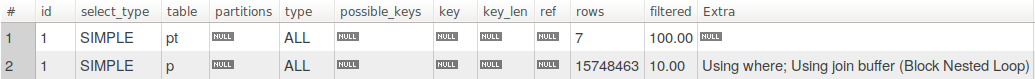
\includegraphics[scale =0.4]{explain14.png} 
	\caption{Przykład 9}
\end{figure}
Dodatkowo należy wziąć pod uwagę, że są to jedynie szacunkowe wartości, które w praktyce mogą być zupełnie nie prawidłowe. Ponadto optymalizator podczas szacowania wartości w kolumnie \textit{rows} nie bierze pod uwagę klauzli \textit{LIMIT}.

\paragraph{Kolumna filtered}\leavevmode\\
Kolumna \textit{filtered} pojawia się jedynie podczas użycia polecenia \textit{EXPLAIN EXTENDED}. Wskazuje na wartość oszacowaną przez optymalizator, która informuje ile rekordów może zostać odfiltrowane za pomocą klauzuli WHERE. W przykładzie 4 optymalizator MySQL oszacował, że jedynie 10 procent użytkowników napisało w sumie więcej niż 10 komentarzy. 

\paragraph{Kolumna extra}\leavevmode\\
Kolumna \textit{extra} zawiera informacje, których nie udało się zamieścić w pozostałych kolumnach. Poniżej przedstawione zostanie kilka najważniejszych informacji, które mogą znaleźć się w tej kolumnie.

\begin{itemize}
	\item 'Using index' - MySQL użyje indeksu pokrywającego zamiast dostępu do tabeli.
	\item 'Using where' - oznacza, że MySQL przeprowadzi filtrowanie danych dopiero po wczytaniu danych z tabeli. Często jest to informacja, która może sugerować zmianę lub stworzenia nowego indeksu bądź całego zapytania.
	\item 'Using temporary' - do sortowania wyników używana jest tabela tymczasowa.
	\item 'Using filesort' - sortowanie nie może skorzystać z istniejących indeksów (nie ma odpowiedniego optymalnego indeksu), więc wiersze są sortowane za pomocą jednego z algorytmów sortowania.
	
\end{itemize}
\section{Architektura MySQL}

\subsection{Obsługa połączeń i wątków}
Serwer MySQL oczekuje na połączenia klientów na wielu interfejsach sieciowych:
\begin{itemize}
\item jeden wątek obsługuje połączenia TCP/IP (standardowo port 3306)
\item w systemach UNIX, ten sam wątek obsługuje połączenia poprzez pliki gniazda
\item w systemie Windows osobny wątek obsługuje połączenia komunikacji międzyprocesorowej
\item w każdym systemie operacyjnym, dodatkowy interfejs sieciowy może obsługiwać połączenia administracyjne. Do tego celu może być wykorzystywany osobny wątek lub jeden z wątków menadżera połączeń.
\end{itemize}

Jeżeli dany system operacyjny nie wykorzystuje połączeń na innych wątkach, osobne wątki nie są tworzone.

Maksymalna ilość połączeń zdefinowana jest poprzez zmienną systemową \underline{max\_connections}, który domyślnie przyjmuje wartość 151. Dodaktowo MySQL jedno połączenie rezerwuje dla użytkownika z uprawnieniami \underline{SUPER} lub \underline{CONNECTION\_ADMIN}. Taki użytkownik otrzyma połączenie nawet w przypadku braku dostępnych połączeń w głównej puli.

Do każdego klienta łączącego się do bazy MySQL przydzielany jest osobny wątek wewnątrz procesu serwera, który odpowiada za przeprowadzenie autentykacji oraz dalszą obsługę połączenia. Co ważne, nowy wątek tworzony jest jedynie w ostateczności. Jeżeli to możliwe, menadżer wątków stara się przydzielić wątek do połączenia, z puli dostępnych w pamięci podręcznej wątków.

\subsection{Bufor zapytań}
Bufor zapytań przechowuje gotowe odpowiedzi serwera dla poleceń SELECT. Jeżeli wynik danego zapytania znajduje się w buforze zapytań, serwer może zwrócić wynik bez konieczności dalszej analizy.

Proces wyszukiwania zapytania w buforze wykorzystuje funkcję skrótu. Dla każdego zapytania tworzony jest hash, który pozwala w prosty sposób zweryfikować, czy dane zapytanie znajduje się w buforze. Co ważne, hash uwzględnia wielkość liter, co prowadzi do sytuacji, gdzie dwa zapytania różniące się jedynie wielkością liter nie zostaną uznane za jednakowe.

Jeżeli tabela, z której pobierane są dane poprzez polecenie SELECT  zostanie zmodyfikowana, wszystkie zapytania odnoszące się do takiej tabeli zostają usunięte z bufora. Dodatkowo bufor zapytań nie przechowuje zapytań uznanych, za niederministyczne. Przykładowo wszystkie polecenia pobierające aktualną datę, użytkownika itp nie zostaną dodane do bufora zapytań. Co istotne nawet w przypadku zapytania niederministycznego, serwer oblicza funkcję skrótu dla zapytania i próbuje dopasować odpowienie zapytanie z tabeli bufora. Dzieje się tak ze względu na fakt, że analiza zapytania odbywa się dopiero po przeszukaniu bufora i na etapie przeszukiwania bufora, serwer nie ma informacji o tym czy zapytanie jest deterministyczne. Jedynym filtrem, który weryfikuje zapytanie przed przeszukaniem bufora, jest sprawdzenie czy polecenie rozpoczyna się od liter SEL.

Jeżeli polecenie SELECT składa się z wielu podzapytań, ale nie znajduje się w tabeli bufora, to żadne z nich nie zostanie pobrane, ponieważ bufor zapytań działa na podstawie całego polecenia SELECT.


\section{Silniki magazynu danych}
Niniejszy rozdział poświęcony jest omówieniu zagadnień związanych z silnikami bazy danych. Silnik bazy danych jest częścią bazy danych odpowiedzialną za wykonywanie kodu SQL, czyli wykonywanie operacji na danych. SQL jest językiem deklaratywnym. Klient podając polecenie SQL, opisuje warunku, jakie musi spełnić końcowe rozwiązanie, a nie szczegółową implementację. Z tego wynika, że to silnik bazy danych odpowiedzialny jest za dostarczenie implementacji pozwalajacej na wykonywanie kodu SQL. Silnik dodatkowo definiuje sposób przechowywania dnaych oraz zbiór operacji, które możemy na nich wykonać.

Architektura MySQL umożliwia korzystanie z wielu różnych silników. Silnik bazy danych wybierany jest per tabela, co oznacza, że w ramach pojedynczej bazy danych można używać różnych silników.
\subsection{Krótka charakterystyka podstawowych silników.}
W tym podrozdziale nie zostały przedstawione szczegółowe opisy silników dostępnych w MySQL, raczej ich główne charakterystyki, zalety oraz ograniczenia. Część z silników pominięto ze względu na ich marginalną popularność oraz zastosowanie. W zdecydowanej większości przypadków aktualnie najodpowiedniejszym silnikiem jest InnoDB, aczkolwiek każdy z silników opisanych w tym rozdziale ma pewne zalety i w specyficznych przypadkach przedstawionych w tym podrozdziale, warto rozważyć użycie silnika alternatywnego do InnoDB.
\subsubsection{MyISAM}
MyISAM był domyślnym silnikiem składowania danych do wersji 5.4 (włącznie). Każda tabela przechowywana jest w dwóch plikach na dysku twardym. Dane przechowywane są w pliku z rozszerzeniem \textbf{.MYD (MYData)}
natomiast w drugim pliku (\textbf{.MYI(MYIndex)}) składowane są indeksy. Poniżej przedstawiono kilka cech tego silnika bazy danych. 
\begin{itemize}
	\item \textbf{Brak wsparcia dla transakcji.} Z tego powodu MyISAM nie powinien być używany do tabel, dla których istotnym wymaganiem jest zapewnienie integralności danych.
	\item \textbf{Obsługa indeksów B-tree oraz Geospatial.}
	\item \textbf{Blokady tabeli.}  W momencie wykonywana operacji dodającej dane do tabeli jest ona blokowana na cały czas wykonywania operacji (również dla operacji odczytujących dane). Sprawia to, że w przypadku dużej liczby operacji modyfikujących dane - wydajność bazy danych wyraźnie spada.
	\item \textbf{Brak obłusgi mechanizmu kluczy obcych}
	\item \textbf{Mechanizm kompresji danych.} Silnik umożliwia kompresowanie danych w celu optymalizacji ilości miejsca potrzebnego do przechowywania danych z tabeli. Taka operacja sprawia, że skompresowane dane są dostępne jedynie do odczytu, a ich modyfikacja jest zablokowana i wymaga rozpakowania danych. Tabele MyISAM można kompresować i dekompresować za pomocą mechanizmu \textit{myisampack}.
	\item \textbf{Buforowanie indeksów.} Silnik MyISAM buforuje jedynie indeksy.
	\item \textbf{Obsługa statystyk.}
\end{itemize}

W czasie pisania tej pracy silnik MyISAM nie był już rozwijany, dlatego raczej odradzane jest jego stosowanie w nowszych wersjach serwera MySQL. 

\subsubsection{InnoDB}
Od wersji 5.5 InnoDB jest domyślnym silnikiem bazy danych MySQL. Mechanizm InnoDB uzupełniono o funkcje, których brakowało w MyISAM i obecnie jest zdecydowanie najpopularniejszym wyborem. Domyślnie dane przechowywane są w pojedynczych plikach, ale możliwe być również przechowywane w wielu plikach. Strukturę plików bazy \textit{StackOverflow}, która dla wszystkich tabel używa silnika InnoDB, przedstawiono na rysunku ~\ref{fig:innodb-fileslabel}.
\begin{figure}
	\caption{Pliki silnika InnoDB testowej bazy danych \textit{StackOverflow}}
	\centering
	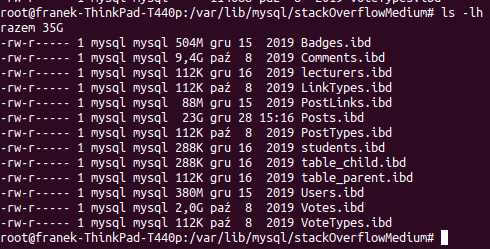
\includegraphics[scale = 0.43]{innodb-files.png}
	\label{fig:innodb-fileslabel}
\end{figure}
Poniżej przedstawiono podstawowe charakterystyki silnika.
\begin{itemize}
	\item \textbf{Wsparcie dla transakcji.} Silnik wspiera transakcje oraz wszystkie cztery poziomy izolacji modelu \textit{ANSI}. Poziom izolacji transakcji określa zasady widoczności pomiędzy współbieżnymi transakcjami. Dzięki wsparciu dla wszystkich czterech izolacji  silnik InnoDB spełnia wymagania stawiane aplikacją wymagającym zapewnienie integralności danych. 
	\item \textbf{Wsparcie dla indeksów.} InnoDb wspiera najważniejsze indeksy takie jak: B-tree, Hash, Spatial.
	\item \textbf{Blokowanie dostępu na poziomie rekordów. } Dostęp do tabel InnoDB jest blokowany za pomocą mechanizmy MVCC (Multi-Versioned Concurrency Control). Blokowane są pojedyncze rekody, zamiast całej tabeli. Wprowadzenie tej zmiany znacząco zwiększyło wydajność równoległych operacji modyfikujących dane w tabeli.
	\item \textbf{Wsparcie dla kluczy obcych.}
	\item \textbf{Buforowanie danych oraz indeksów.} Silnik InnoDb może buforować nie tylko indeksy, ale również dane.
	\item  \textbf{Nieskompresowane indeksy.} Silnik InnoDb nie kompresuje indeksów, co prowadzi do zwiększenia zużycia przestrzeni dyskowej.
	\item \textbf{Wsparcie dla partycjonowania.} Szerzej opisane w podrozdziale dotyczącym partycjonowania.
	\item \textbf{Obsługa statystyk.}
\end{itemize}

\subsubsection{CSV Storage Engine}
Silnik CSV Storage Engine przechowuje dane tabeli w plikach tekstowych w formacie csv z wartościami rozdzielonymi przecinkami.Ten silnik może być przydatny, jeżeli chcemy nasze dane przechowywać w formacie csv. Posiada wiele ograniczeń, dlatego nie jest zalecane jego stosowanie, o ile nie zależy nam na przechowywaniu danych tabeli w formacie CSV.
Poniżej przedstawiono podstawowe ograniczenia tego silnika.
\begin{itemize}
	\item \textbf{Brak wsparcia dla indeksów i kluczy obcych.}
	\item \textbf{Brak wsparcia dla transakcji.}
	\item \textbf{Brak możliwości przechowywania wartości \textit{null}.}
	\item \textbf{Brak wsparcia dla partycjonowania.}
\end{itemize}

\subsubsection{Memory}
Silnik Memory przechowuje wszystkie dane w pamięci, a nie na dysku twardym. Te dane są ulotne i zostają usunięte w momencie restartu serwera (struktura tabeli zostaje zachowana). Z powodu przechowywania w pamięci są o rząd wielkości szybsze od standardowych silników baz danych, ale ze względu na swoją ulotność nie powinny przechowywać istotnych danych dla aplikacji.
Poniżej przedstawiono podstawowe własności tabeli Memory.
\begin{itemize}
	\item \textbf{Wsparcie dla indeksów} Tabele Memory obsługują indeksy Hash oraz B-tree. Domyślnym indeksem jest indeks typ Hash.
	\item \textbf{Blokowanie na poziomie tabeli.} Podobnie jak tabele MyISAM, w momencie modyfikowania danych blokowana jest cała tabela.
	\item \textbf{Brak obsługi typów TEXT oraz BLOB}. Tabele nie obsługują typów TEXT. Przechowywanie teksu możliwe jest w kolumnach VARCHAR o stałej zdefiniowanej wielkości, co prowadzi do marnotrawienia pamięci.
	\item \textbf{Brak danych statystycznych indeksu.} Tabele MEMORY nie przechowują statystyk dotyczących indeksów, co czasami może skutkować wybraniem nieodpowiedniego indeksu przez optymalizator zapytań i w efekcie pogorszenie wydajności zapytań.
	\item \textbf{Brak wsparcia dla transakcji.}
\end{itemize}

Zastosowanie silnika MEMORY warto rozważyć w następujących sytuacjach.
\begin{itemize}
	\item Pamięć podręczna dla często odczytywanych danych, która jest wczytywana w momencie startu serwera.
	\item Buforowanie wyników agregowanych danych z często wykonywanych zapytań.
	\item Przechowywanie wyników pośrednich z zapytań.
	\item MySQL używa tabeli Memory do wewnętrznego przetwarzania zapytań wymagających tabeli tymczasowych do przechowywania wyników pośrednich.
\end{itemize}

\subsubsection{Silnik Archive}
Archive jest silnikiem służącym do przechowywania dużej ilości nieindeksowanych danych, które są rzadko pobierane. 

Podstawowe cechy tego silnika zostały przedstawione poniżej.
\begin{itemize}
	\item \textbf{Brak wsparcia dla transakcji.}
	\item \textbf{Możliwe wykonywanie jedynie operacji INSERT, REPLACE oraz SELECT}. W tabelach Archive niemożliwe jest usuwanie i modyfikowanie istniejących krotek.
	\item \textbf{Brak wsparcia dla indeksów.}
	\item \textbf{Blokowanie na poziomie tabeli.}
	\item \textbf{Kompresowanie danych.} Każdy wstawiony rekord jest automatycznie kompresowany za pomocą \textit{zlib}, dlatego tabele Archive wymagają zdecydowanie mniej miejsca od tabel InnoDB lub MyISAM.
\end{itemize}


\subsection{Porównanie silników}



\subsubsection{Przechowywanie danych}
W celu porównania sposobu przechowywania danych na dysku przegotowano testową bazę danych, zawierającą pięć tabel będących niemalże kopią tabeli \textit{Users} z bazy testowej, z których każda wykorzystuje inny silnik. Jedyną zmianą jest brak kolumny \textit{AboutMe}, która została usunięta ze względu brak wsparcia dla kolumn TEXT w silniku MEMORY. Do tworzenia tabel wykorzystano polecenia z poniższego listingu, a następnie zaimportowano dane z bazy \textit{Stackoverflow}. Ponieważ nie wszystkie silniki wspierają przechowywania wartości NULL, zamieniono domyślne wartości NULL na wartość 0 lub pusty tekst (w zależności od typu danych).
\begin{spverbatim}
	CREATE TABLE `Users` (
	`Id` int NOT NULL,
	`Age` int NOT NULL DEFAULT 0,
	`CreationDate` datetime NOT NULL,
	`DisplayName` varchar(80) NOT NULL,
	`DownVotes` int NOT NULL,
	`EmailHash` varchar(80) NOT NULL DEFAULT '',
	`LastAccessDate` datetime NOT NULL,
	`Location` varchar(200) NOT NULL DEFAULT '',
	`Reputation` int NOT NULL,
	`UpVotes` int NOT NULL,
	`Views` int NOT NULL,
	`WebsiteUrl` varchar(400) NOT NULL DEFAULT '',
	`AccountId` int NOT NULL DEFAULT 0,
	PRIMARY KEY (`Id`) -- w tabelach, które wspierają klucze główne
	) ENGINE=<nazwa silnika>;
\end{spverbatim}
Klucze główne zostały usunięte w przypadku silników, które ich nie wspierają. Ostatecznie tabela zawiera około 2,5 miliona wierszy.
\begin{figure}[!h]
	\caption{Baza danych użyta do testowania silników baz danych}
	\centering
	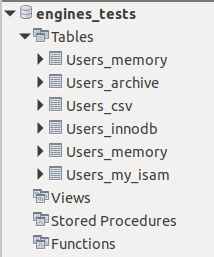
\includegraphics[scale = 0.59]{engines_tests.png}
	\label{fig:label}
\end{figure}
\begin{figure}[!h]
	\caption{Pliki z danymi użytkowników dla testowych silników.}
	\centering
	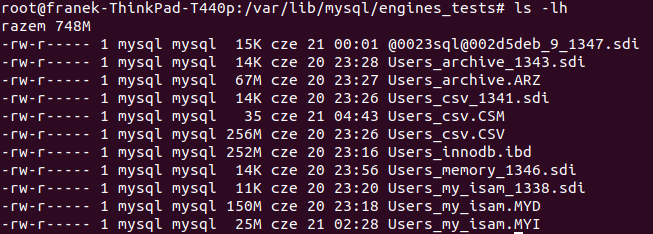
\includegraphics[scale = 0.6]{engines_storage.png}
	\label{fig:engines_storage}
\end{figure}

Na rysunku ~\ref{fig:engines_storage} przedstawiono pliki tabel testowej bazy danych. Pod względem optymalizacji ilości miejsca na dysku zdecydowanie najlepiej wypada silnik Archive, który potrzebuje jedynie 67 MB dla danych użytkowników. Na drugim miejscu pod tym względem plasuje się silnik MyISAM. Silniki InnoDB oraz CSV wymagają praktycznie takiej samej przestrzeni dyskowej; w granicach 250 MB. Silnik MEMORY na dysku twardym przechowuje jedynie strukturę tabeli, ale do sprawdzenia ilości użytej pamięci możemy użyć narzędzia \textit{MySQL Workbench}.
\begin{figure}[!h]
	\caption{Informacje dotyczące tabeli Users\textunderscore memory w \textit{MySQL Workbench}. \textit{StackOverflow}}
	\centering
	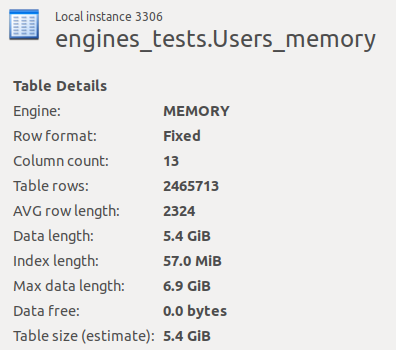
\includegraphics[scale = 0.6]{memory_engine_storage.png}
	\label{fig:label}
\end{figure}
Silnik MEMORY wymaga prawie 5.5 Gb pamięci. Wynika to w dużej mierze z tego, że silnik MEMORY dla kolumn VARCHAR zawsze rezerwuje rozmiar wynikający z maksymalnej wartości, nawet jeżeli nie jest ona wykorzystana.




\subsubsection{Wymaganie transakcyjności}
W przypadku tabel, które wymagają użycia transakcji, jedynym możliwym wyborem jest silnik InnoDB.

\subsubsection{Operacje odczytu klucz-wartość}
Do testowania użyto narzędzia \textit{sysbench}, które posiada wbudowany mechanizm ułatwiający testowanie baz danych. Za pomocą poniższych poleceń rzygotowano testową bazę danych udostępnioną przez \textit{sysbench}. 
\begin{spverbatim}
	sysbench --db-driver=mysql --mysql-user=root --mysql-password=root --mysql-db=test --table_size=2000000 --range_selects=off --mysql_storage_engine=
	<nazwa silnika> /usr/share/sysbench/oltp_read_only.lua prepare
\end{spverbatim} 
Baza danych zawiera 2 miliony rekordów, tabela domyślnie przyjmuje nazwę \textit{sbtest1}.
\begin{figure}[H]
	\caption{Struktura tabeli \textit{sbtest1}.}
	\centering
	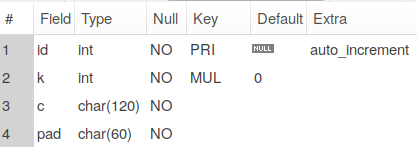
\includegraphics[scale = 0.6]{struktura_sbtest1.png}
	\label{fig:label}
\end{figure}

Aby wykonać test polecenie \textit{prepare} należy zamienić na polecenie \textit{run}. Przy takiej konfiguracji wykonywane jest następujące zapytanie:
\begin{spverbatim}
	SELECT c FROM sbtest1 WHERE id=?
\end{spverbatim}
\begin{figure}[H]
	\caption{Przykładowe statystyki testu wydajności izolowanych operacji odczytu.}
	\centering
	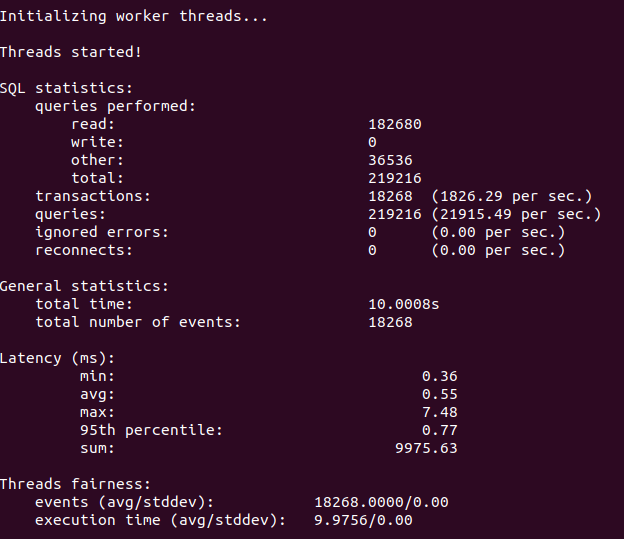
\includegraphics[scale = 0.6]{sysbench_statistics.png}
	\label{fig:label}
\end{figure}
\begin{center}
	\begin{tabular}{ | c | c | c | c | c | c |}
		\hline
		- & MyISAM & InnoDB & Memory & Archive & CSV  \\ 
		\hline
		średni czas [ms] & 0.54 & 0.55 & 0.38 & powyżej minuty & powyżej minuty \\
		\hline
	\end{tabular}
\end{center}
Z powyższej tabeli wynika, że w przypadku zapytań używających pełnego klucza głównego, silnik MEMORY jest najwydajniejszy. Dobry wynik wynika z faktu zastosowania indeksu HASH na kolumnie Id. Silniki InnoDB oraz MyISAM prezentują podobną wydajność w przypadku zapytań używających indeksy (w tym przypadku indeksy BTree). Silniki Archive oraz CSV wyraźnie odstają w tym zestawieniu ze względu na brak obsługi kluczy głównych.


\subsubsection{Symultaniczne operacje odczytu z wykorzystaniem klucza głównego oraz operacji zapisu.}

Do przygotowania testowych zestawów danych wykorzystano następujące skrypty:
\begin{spverbatim}
	sysbench --db-driver=mysql --mysql-user=root --mysql-password=root --mysql-db=test --table_size=2000000 --num-threads=12 --range_selects=off --mysql_storage_engine=<nazwa silinika>  /usr/share/sysbench/oltp_read_write.lua prepare
\end{spverbatim}

Wykonanie testu analogicznie jak w poprzednich przypadkach wykonano, zastępując słowo kluczowe \textit{prepare} na \textit{run}.


Na rysunku ~\ref{fig:wyniki_testu_symulatnicznych_odczytow} przedstawiono wyniki testu. W przypadku tego testu operacje odczytu wykonywane były równolegle z operacjami zapisu do tabeli.
\begin{figure}[H]
	\caption{Przykładowe statystyki testu symultanicznych odczytów i zapisów.}
	\centering
	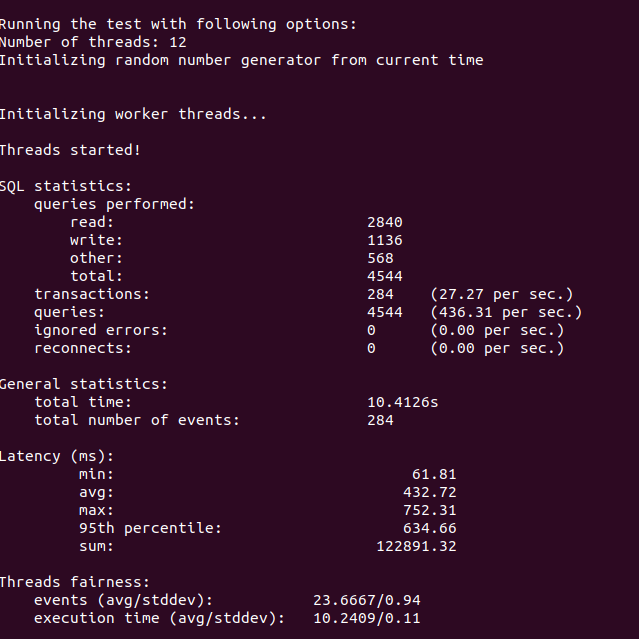
\includegraphics[scale = 0.6]{wyniki_testu_symulatnicznych_odczytow.png}
	\label{fig:wyniki_testu_symulatnicznych_odczytow}
\end{figure}
\begin{center}
	\begin{tabular}{ | c | c | c | c | c | c |}
		\hline
		- & MyISAM & InnoDB & Memory & Archive & CSV  \\ 
		\hline
		średni czas [ms] & 432.7 & 75.5 & 425.1 & powyżej minuty & powyżej minuty \\
		\hline
	\end{tabular}
\end{center}
Wyniki testu przedstawione w tabeli powyżej wskazują, że najwydajniejszym silnikiem w przypadku równoleglych operacji odczytu i modyfikacji danych w środowisku wielowątkowym okazał się silnik InnoDB, na co wpływ ma zastosowanie mechanizmu blokowania pojedynczych rekordów, zamiast całej tabeli zastosowany w pozostałych.

\subsubsection{Wyszukiwanie danych z zakresu.}
Kolejny test symuluje operację wyszukiwania danych za pomocą zakresu. Do jego przygotowania wykorzystano następujące polecenie.
\begin{spverbatim}
	sysbench --db-driver=mysql --mysql-user=root --mysql-password=root --mysql-db=test --table_size=2000000 --mysql_storage_engine=<nazwa silniku> --num-threads=12 /usr/share/sysbench/select_random_ranges.lua prepare
\end{spverbatim}
W związku z tym, że domyślnym indeksem dla tabeli MEMORY jest indeks HASH, a nie B-tree, na tej tabeli dodatkowo utworzono indeks typu B-Tree, wykorzystując następujące polecenie.
\begin{spverbatim}
	CREATE INDEX k_12 on sbtest1(k) USING btree;
\end{spverbatim}
\begin{center}
	\begin{tabular}{ | c | c | c | c | c | c |}
		\hline
		- & MyISAM & InnoDB & Memory & Archive & CSV  \\ 
		\hline
		średni czas [ms] & 1.23 & 1.25 & 0.51 & 26687 & 51400 \\
		\hline
	\end{tabular}
\end{center}

Wyniki testu pokazują, że przy tego typu operacjach najwydajniejsze są silniki wykorzystujące indeksy typu B-Tree, które pozwalają w optymalny sposób wyszukiwać za pomocą zakresu. Silnik \textit{MEMORY} okazał się najszybszy ze względu na przechowywanie danych bezpośrednio w pamięci.

\subsubsection{Operacje zapisu.}
Kolejny test prezentuje wydajność operacji zapisu w środowisku wielowątkowym. Do jego wykonania użyto następującego polecenia:
\begin{spverbatim}
	 sysbench --db-driver=mysql --mysql-user=root --mysql-password=root --mysql-db=test --table_size=2000000 --mysql_storage_engine=<nazwa silnika> --num-threads=12 /usr/share/sysbench/oltp_insert.lua prepare
\end{spverbatim}

Wyniki testu przedstawiono w poniższej tabeli:
\begin{center}
	\begin{tabular}{ | c | c | c | c | c | c |}
		\hline
		- & MyISAM & InnoDB & Memory & Archive & CSV  \\ 
		\hline
		średni czas [ms] & 107.8 & 37.9 & 104.1 & 17.1 & 108.9 \\
		\hline
	\end{tabular}
\end{center}

W teście najszybszy okazał się silnik \textit{Archive}, który został zaprojektowany właśnie do wydajnego zapisywania danych. Znaczny wpływ na dużą wydajność ma fakt braku indeksów. Dzięki temu serwer nie spędza dodatkowego czasu na aktualizacji indeksu podczas wstawiania nowych krotek. Istotna jest również niemal trzykrotnie większej wydajność operacji zapisu w tabelach \textit{InnoDB} w porównaniu do \textit{MyISAM} i \textit{MEMORY}. Jest to wynikiem zastosowania blokowania na poziomie rekordu.

\subsubsection{Operacje aktualizacji danych z wykorzystaniem indeksu.}

Kolejny test przedstawia wydajność operacji aktualizacji danych z wykorzystaniem indeksu w środowisku wielowątkowym. Do jego przygotowania użyto następującego polecenia.
\begin{spverbatim}
	sysbench --db-driver=mysql --mysql-user=root --mysql-password=root --mysql-db=test --table_size=2000000 --num-threads=12 --mysql-storage_engine=
	<nazwa silnika> /usr/share/sysbench/oltp_update_index.lua prepare
\end{spverbatim}

Wyniki testu zamieszczono w poniższej tabeli.
\begin{center}
	\begin{tabular}{ | c | c | c | c | c | c |}
		\hline
		- & MyISAM & InnoDB & Memory & Archive & CSV  \\ 
		\hline
		średni czas [ms] & 109.1 & 54.9 & 105.9 & Brak wsparcia & Brak indeksów \\
		\hline
	\end{tabular}
\end{center}

Test jest miarodajny jedynie dla trzech silników wspierających indeksy. Podstawową przyczyną powodującą niemal dwukrotnie większą wydajność operacji modyfikujących dane w silniku \textit{InnoDB}, jest mechanizm blokowania na poziomie rekordów.

\subsubsection{Operacje aktualizacji danych bez wykorzystania indeksów.}
Kolejny test również przedstawia wydajność operacji aktualizacji danych w środowisku wielowątkowym, ale bez wykorzystania indeksów.
Do wykonania testu użyto polecenia:
\begin{spverbatim}
	sysbench --db-driver=mysql --mysql-user=root --mysql-password=root --mysql-db=test --table_size=2000000 --num-threads=12 --mysql-storage_engine=
	<nazwa silnika> /usr/share/sysbench/oltp_update_non_index.lua prepare
	
\end{spverbatim}
\begin{center}
	\begin{tabular}{ | c | c | c | c | c | c |}
		\hline
		- & MyISAM & InnoDB & Memory & Archive & CSV  \\ 
		\hline
		średni czas [ms] & 107.6 & 46.9 & 107.1 & Brak wsparcia & 67627.1 \\
		\hline
	\end{tabular}
\end{center}

Testy potwierdzają, że w środowisku wielowątkowym przy operacjach modyfikujących dane najwydajniejszy jest silnik \textit{InnoDB}, dzięki blokowaniu na poziomie rekordów.
\subsubsection{Operacje usuwania danych}
W kolejnym teście sprawdzono wydajność operacji usuwania danych w środowisku wie
\begin{spverbatim}
	sysbench --db-driver=mysql --mysql-user=root --mysql-password=root --mysql-db=test --table_size=2000000 --num-threads=12 --mysql-storage_engine=<nazwa tabeli>  /usr/share/sysbench/oltp_delete.lua prepare
\end{spverbatim}

\begin{center}
\begin{tabular}{ | c | c | c | c | c | c |}
	\hline
	- & MyISAM & InnoDB & Memory & Archive & CSV  \\ 
	\hline
	średni czas [ms] & 312.5 & 43.3 & 106.1 & Brak wsparcia & 62342.1 \\
	\hline
\end{tabular}

Silnik InnoDB jest najwydajniejszym rozwiązaniem ze względu na mechanizm blokowania na poziomie rekordów.
\end{center}


\subsubsection{Podsumowanie}

W tym rozdziale przedstawiono podstawowe własności najpopularniejszych dostępnych obecnie silników MySQL. W zdecydowanej większości przypadków, które możemy spotkać we współczesnych aplikacjach, korzystających z baz danych najlepszym rozwiązaniem jest silnik InnoDB. W przypadku tabel, do których dane są jedynie zapisywane, ale nie odczytywane, dobrym wyborem jest silnik \textit{Archive}, który zapewnia najlepszą wydajność operacji zapisu, oraz zdecydowanie niższe zużycie przestrzeni dyskowej od pozostałych silników. Wyniki testów wydajnościowych potwierdzają, że silnik \textit{MyISAM} nie powinien być obecnie stosowany. Silnik \textit{InnoDB} będący jego następcą jest bardziej wydajny, a dodatkowo zawiera mechanizmy, których brakuje \textit{MyISAM}. Silnik \textit{MEMORY} w środowisku wielowątkowym nie jest bardziej wydajny od \textit{InnoDB}, a dodatkowo zużywa wiele pamięci. Silnik \textit{CSV} jest niewydajny i ubogi w funkcje, dlatego według autora nie powinien być używany w produkcyjnych zastosowaniach.
\section{Optymalizator MySQL}

Zasadniczo każde zapytanie SQL skierowane do bazy danych MySQL może zostać zrealizowane na wiele różnych sposobów. Optymalizator jest fragmentem oprogramowania serwera MySQL, który odpowiada za wybranie najefektywniejszego sposobu wykonania zapytania (plan wykonania zapytania).
Proces ten ma kilka etapów. W pierwszej kolejności analizator MySQL dzieli zapytanie na tokeny i z nich tworzy "drzewo analizy". Na tym etapie przeprowadzana jest jednocześnie analiza składni zapytania. Następnym krokiem jest \textit{preprocessing}, w którego trakcie sprawdzane są między innymi: nazwy kolumn i tabel, a także nazwy i aliasy, aby zapewnić, że nazwy użyte w zapytaniu nie są np. dwuznaczne. Na kolejnym etapie weryfikowane są uprawnienia. Czynność ta może zajmować szczególnie dużo czasu, jeżeli serwer posiada ogromną liczbę uprawnień. Po zakończeniu etapu \textit{preprocessingu} drzewo analizy jest poprawne i gotowe do tego, aby optymalizator przekształcił je do postaci planu wykonania.

W MySQL stosowany jest optymalizator kosztowy, co oznacza, że optymalizator szacuje koszt wykonania dla wariantów planu wykonania i wybiera ten z najmniejszym kosztem. Jednostką kosztu jest odczytanie pojedynczej, losowo wybranej strony danych o wielkości czterech kilobajtów. Wartość kosztu jest wyliczana na podstawie danych statystycznych, dlatego optymalizator wcale nie musi wybrać optymalnego planu. Istnieją dwa rodzaje optymalizacji: \textit{statyczna} i \textit{dynamiczna}. Optymalizacja \textit{statyczna} przeprowadzana jest tylko raz i jest niezależna od wartości używanych w zapytaniu. To oznacza, że przeprowadzona raz będzie aktualna, nawet jeżeli zapytanie będzie wykonywane z różnymi wartościami. Natomiast optymalizacja dynamiczna bazuje na kontekście, w którym wykonywane jest zapytanie i jest przeprowadzana za każdym razem, kiedy polecenie jest wykonywane. Optymalizacja dynamiczna opiera się na wielu parametrach, takich jak: wartości w klauzuli WHERE czy liczba wierszy w indeksie, które znane są dopiero w momencie wykonania zapytania.

Poniżej przedstawione zostało kilka przykładowych optymalizacji, które może wykonać moduł serwer MySQL.

\begin{itemize}
	\item \textbf{Zmiana kolejności złączeń}. Podczas wykonywania zapytania tabele nie zawsze są łączone w takiej kolejności jak w zapytaniu. Zagadnienie jest dokładniej opisane w podrozdziale dotyczącym optymalizatora złączeń.
	\item \textbf{Zamiana OUTER JOIN na INNER JOIN.} Nawet jeżeli w zapytaniu użyjemy klauzuli OUTER JOIN, złączenie nie zawsze musi być wykonywany jako OUTER JOIN. Niektóre czynniki takie jak warunki w klauzuli WHERE czy schemat bazy danych mogą spowodować, że OUTER JOIN będzie równoznaczne złączeniu INNER JOIN. 
	\item \textbf{Przekształcenia algebraiczne.} Optymalizator przeprowadza transformacje algebraiczne takie jak: redukcja stałych, eliminowanie nieosiągalnych warunków czy stałych. Przykładowo warunek (2=2 AND a>2) może zostać przekształcony do postaci (a>2). Podobnie warunek (a<b AND b=c AND a=5) może być przekształcony do (b>5 AND b=c AND a=5).
	\item \textbf{Optymalizacja funkcji MIN(), MAX().}
	Serwer już na etapie optymalizacji zapytania może uznać wartości zwracane przez funkcje jako stałe dla reszty zapytania. W niektórych przypadkach optymalizator może nawet pominąć tabelę w planie wykonania zapytania, jeżeli jedyną wartością pobieraną z tabeli jest wynik funkcji MIN() lub MAX(). W takim przypadku w danych wyjściowych polecenia EXPLAIN znajdzie się ciąg tekstowy''Select tables optimized away''.
	Na rysunku ~\ref{fig:explain20} widzimy, że kolumna \textit{ref} dla pierwszego wiersza jest wartość ''const'', czyli najmniejsza wartość id z tabeli \textit{Users} została potraktowana jako stała.
	\begin{spverbatim}
		EXPLAIN SELECT * FROM Comments WHERE UserId = (SELECT MIN(id) FROM Users);
	\end{spverbatim}
\begin{figure}
	\caption{Pliki silnika InnoDB testowej bazy danych \textit{StackOverflow}}
	\centering
	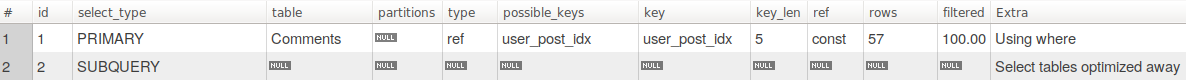
\includegraphics[scale = 0.37]{explain20.png}
	\label{fig:explain20}
\end{figure}
	\item \textbf{Optymalizacja funkcji COUNT().} Wyniki funkcji COUNT() bez klauzuli WHERE w niektórych silnikach (np. MyISM), również mogą zostać potraktowane jako stała, ale nie dotyczy to najpopularniejszego obecnie w MySQL silnika InnoDB.
	\textbf{Optymalizacja stałej tabeli}
	
	\item \textbf{Stałe tabele.} \textit{Stała tabela} jest to tabela, która zawiera co najwyżej jeden wiersz lub warunek zawarty w klauzuli WHERE odnosi się do wszystkich kolumn klucza głównego, albo do indeksu UNIQUE NOT NULL. W takim przypadku MySQL może zwrócić wartość jeszcze przed wykonaniem zapytania i potraktować jako stałą dla dalszej części zapytania.
\end{itemize}

\subsection{Dane statystyczne dla optymalizatora}
Przechowywaniem danych statystycznych jest zadaniem silników bazy danych. Z tego powodu w zależności od użytego silnika przechowywane wartości statystyczne mogą być różne. Przykładowo silnik MyISM przechowuje informację o aktualnej liczbie rekordów w tabeli, a InnoDB takiej informacji nie przechowuje, natomiast niektóre silniki, np. Archive, wcale nie przechowują danych statystycznych.

\subsection{Plan wykonania zapytania}
Wynikiem optymalizacji jest plan wykonania zapytania. Plan wykonania jest zapisywany w postaci drzewa instrukcji, które kolejno wykonywane doprowadzą do zwrócenia wyniku zapytania.
\begin{spverbatim}
	SELECT * FROM Posts p LEFT JOIN PostTypes pt ON p.PostTypeId = pt.Id LEFT JOIN PostLinks pl ON p.Id = pl.PostId LEFT JOIN LinkTypes lt on pl.LinkTypeId = lt.id WHERE PostID = 9;
\end{spverbatim}
Gdybyśmy mieli wyobrazić sobie sposób łączenia tabel w MySQL dla takiego zapytania, zapewne przedstawilibyśmy to tak, jak na poniższym schemacie.
 \begin{center}
 	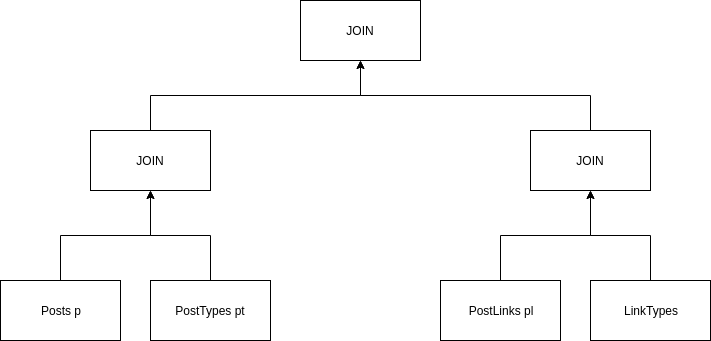
\includegraphics[scale =0.45]{PLAN_WYKONANIA_1.png} 
 \end{center}
W praktyce drzewo instrukcji przybiera postać \textit{drzewa lewostronnie zagnieżdżonego}, co pokazano na rysunku poniżej.
\begin{center}
	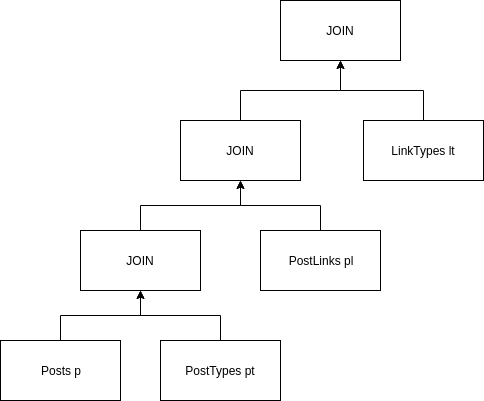
\includegraphics[scale =0.45]{PLAN_WYKONANIA_2.png} 
\end{center}
Wywołując polecenie EXPLAIN dla naszego zapytania, używając klienta \textit{MySQL Workbench} możemy wyświetlić graficzną postać odpowiadającą drzewu instrukcji.
\begin{center}
	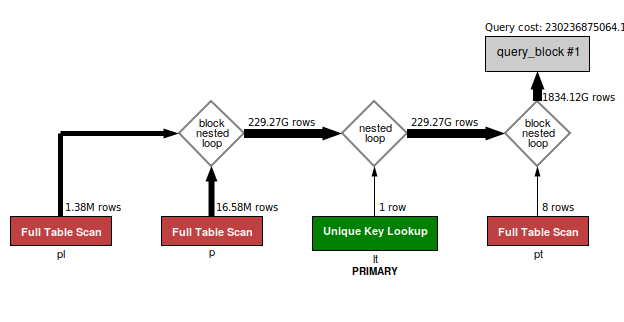
\includegraphics[scale =0.5]{explain21.png} 
\end{center}
Widzimy, że drzewo otrzymane jako wynik polecenia EXPLAIN jest drzewem lewostronnie zagnieżdżonym. Możemy zauważyć też, że optymalizator zdecydował się zamienić kolejność złączeń, aby zminimalizować koszt wykonania zapytania.

\subsection{Optymalizator złączeń}
Większość operacji złączeń można wykonać na wiele różnych sposobów, uzyskując ten sam wynik. Zamiana kolejności jest bardzo skuteczną formą optymalizacji zapytań. Rozważmy teraz następujące przykładowe zapytanie:

\begin{spverbatim}
	SELECT u.Id, p.Id, c.Id, pt.`Type` FROM Users u INNER JOIN Posts p ON u.Id = p.OwnerUserId	INNER JOIN Comments c ON c.UserId = u.Id INNER JOIN PostTypes pt ON pt.Id = p.PostTypeId WHERE u.Id = 4;
\end{spverbatim}

Wykonując polecenie z prefiksem EXPLAIN, otrzymujemy następujący wynik:
\begin{center}
	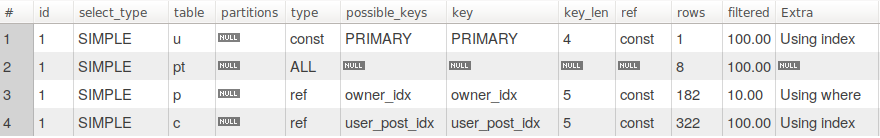
\includegraphics[scale =0.45]{explain22.png} 
\end{center}
Następnie modyfikujemy zapytanie dodając słowo kluczowe STRAIGHT\textunderscore JOIN, aby wymusić kolejność złączeń taką jak w zapytaniu.
\begin{center}
	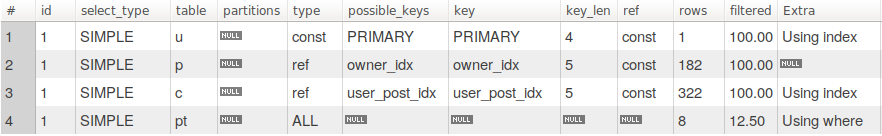
\includegraphics[scale =0.45]{explain23.png} 
\end{center}
Widzimy, że oba rezultaty polecenia są niemalże identyczne, jedyną różnicą jest kolejność dokonywanych złączeń. Sprawdźmy teraz, jaki jest koszt wykonania obu zapytań. Koszt pierwszego zapytania, którego kolejność została zamieniona na etapie optymalizacji, wynosi 6510. Koszt drugiego zapytania wynosi 66868! Zamiana kolejności złączeń zmniejszyła koszt dziesięciokrotnie.
W kolejnym kroku włączyłem profilowanie zapytań za pomocą komendy:
\begin{spverbatim}
	SET PROFILING = 1;
\end{spverbatim}, wykonałem 10 zapytań dla każdego wariantu i policzyłem średni czas, jaki serwer MySQL spędzał na etapie ''executing'', czyli etapie faktycznego wykonywania zapytania. Dla zapytania z kolejnością wybraną przez optymalizator otrzymałem wartość 0.04 sekundy, natomiast przy kolejności wybranej przez nas w zapytaniu wartość ta wynosiła już 0.28 sekundy. Powyższy eksperyment pokazuje, że zamiana kolejności złączeń jest bardzo skuteczną formą optymalizacji i może prowadzić do wielokrotnego zmniejszenia kosztu zapytania. Oczywiście nadal może się zdarzyć sytuacja, kiedy zapytanie z wymuszoną kolejnością załączeń będzie wydajniejsze, ponieważ optymalizator MySQL nie zawsze może sprawdzić wszystkie potencjalne kombinacje złączeń, ale w zdecydowanej większości przypadków optymalizator złączeń okazuje się skuteczniejszy od człowieka.

\subsection{Konfiguracja optymalizatora złączeń}
Optymalizator złączeń stara się wygenerować plan zapytań o najniższym możliwym koszcie. W idealnym przypadku optymalizator zweryfikowałby wszystkie możliwe kombinacje złączeń. Niestety operacja łączenia dla \textit{n} tabel będzie miała \textit{n!} możliwych kombinacji. Oznacza to, że dla dziesięciu tabel złączenia mogą zostać przeprowadzone na 3628800 różnych sposobów i gdyby optymalizator zdecydował się przetestować każdy dostępny scenariusz, kompilacja mogłaby zająć wiele godzin, a nawet dni. Do zdefiniowania, jak wiele planów powinien przetestować optymalizator służy opcja \textit{optimizer\textunderscore search\textunderscore depth}. Na ogół im niższa wartość zmiennej, tym szybciej optymalizator zwróci plan wykonania, ale zmniejsza się też prawdopodobieństwo optymalności planu. Wartość 0 oznacza, że MySQL dla każdego zapytania dobierze odpowiednią (zdaniem optymalizatora) przestrzeń przeszukiwania.

Aby pokazać wpływ parametru \textit{optimizer\textunderscore search\textunderscore depth} przygotowałem następujący kod SQL, który tworzy dwie tabele, a następnie wypełnia je losowymi danymi.

\begin{spverbatim}
	CREATE TABLE `lecturers`
	(
	`id` INT(11) NOT NULL AUTO_INCREMENT,
	PRIMARY KEY (`id`)
	);
	CREATE TABLE `students`
	(
	`id` INT(11) NOT NULL AUTO_INCREMENT,
	`lecturer_id` INT(11) NOT NULL,
	`value` SMALLINT(6) NOT NULL,
	PRIMARY KEY (`id`),
	INDEX `lecturer_id` (`lecturer_id`),
	INDEX `value` (`value`)
	);
	INSERT INTO `lecturers` VALUES (1), (2);
	
	delimiter ;;
	CREATE PROCEDURE fill_tables()
	BEGIN
		DECLARE i int DEFAULT 0;
		WHILE i <= 1000 DO
			INSERT INTO `students` (`id`, `lecturer_id`, `value`) VALUES (0, 1, i);
			INSERT INTO `students` (`id`, `lecturer_id`, `value`) VALUES (0, 2, i);
			SET i = i + 1;
		END WHILE;
	END;;
	delimiter ;
	
	CALL fill_tables();
\end{spverbatim}

W kolejnym kroku wykonałem wielokrotnie następujące zapytanie:
\begin{spverbatim}
	SELECT COUNT(*) FROM table_parent AS p WHERE 1
	AND EXISTS (SELECT 1 FROM students AS s WHERE s.lecturer_id = p.id AND s.value = 1 LIMIT 1)
	AND EXISTS (SELECT 1 FROM students AS s WHERE s.lecturer_id = p.id AND s.value = 2 LIMIT 1)
	AND EXISTS (SELECT 1 FROM students AS s WHERE s.lecturer_id = p.id AND s.value = 3 LIMIT 1)
	AND EXISTS (SELECT 1 FROM students AS s WHERE s.lecturer_id = p.id AND s.value = 4 LIMIT 1)
	AND EXISTS (SELECT 1 FROM students AS s WHERE s.lecturer_id = p.id AND s.value = 5 LIMIT 1)
	AND EXISTS (SELECT 1 FROM students AS s WHERE s.lecturer_id = p.id AND s.value = 6 LIMIT 1)
	AND EXISTS (SELECT 1 FROM students AS s WHERE s.lecturer_id = p.id AND s.value = 7 LIMIT 1)
	AND EXISTS (SELECT 1 FROM students AS s WHERE s.lecturer_id = p.id AND s.value = 8 LIMIT 1)
	AND EXISTS (SELECT 1 FROM students AS s WHERE s.lecturer_id = p.id AND s.value = 9 LIMIT 1)
	AND EXISTS (SELECT 1 FROM students AS s WHERE s.lecturer_id = p.id AND s.value = 10 LIMIT 1)
\end{spverbatim}
zmieniając parametr \textit{optimizer\textunderscore search\textunderscore depth}, dla każdej wartości zmiennej zapisałem średni czas wykonania polecenia EXPLAIN. Wyniki umieściłem w poniższej tabeli.

\begin{center}
	\begin{tabular}{ |c|c| } 
		\hline
		optimizer\textunderscore search\textunderscore depth & czas [sekund]\\ 
		\hline
		0 & 1.8\\
		1 & 0.0011\\
		2 & 0.0019\\
		3 & 0.0059\\
		5 & 0.6\\
		10 & 15\\
		20 & 22\\
		30 & 27\\
		62 & 36\\
		\hline
	\end{tabular}
\end{center}
Widzimy, że wraz ze wzrostem wartości parametru wzrastał czas wykonywania polecenia SQL. Kolejnym krokiem było włączenie profilowania i sprawdzenie, na który z etapów serwer spędził najwięcej czasu. Wyniki zostały posortowane według czasu i na poniższym zrzucie ekranu widzimy profil zapytania dla wartości 62.
\begin{center}
	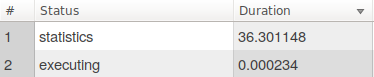
\includegraphics[scale =0.60]{profile1.png} 
\end{center}
Profilowanie zapytania wskazuje nam, że przez większość czasu zapytania, serwer starał się zebrać dane, które pozwolą mu wybrać optymalny plan wykonania zapytania. Obserwacja pokazuje, że dla pewnych zapytań, próba wybrania optymalnego rozwiązania może skończyć się gigantycznym wydłużeniem czasu zapytania. Co ciekawe nawet dla wartości 0 optymalizacja okazał się nieefektywna, co prowadzi do wniosku, że czasami jedym rozwiązaniem w przypadku, kiedy serwer zbyt dużą ilość czasu spędza na szukaniu optymalnego planu, jest ręczna zmiana wartości parametru \textit{optimizer\textunderscore search\textunderscore depth}.

Drugim atrybutem, który służy do konfiguracji optymalizatora złączeń jest \textit{optimizer\textunderscore prune\textunderscore level}. Parametr decyduje o tym, czy optymalizator może wykorzystać heurystyki do wybrania optymalnego planu. Jeżeli ta opcja zostanie włączona, optymalizator może pominąć niektóre plany, bazując na pewnych heurystykach. Dokumentacja MySQL wskazuje, że relatywnie rzadko dochodzi do sytuacji, kiedy optymalizator pomija optymalny plan wykonania, a włączenie tej opcji może znacznie przyśpieszyć proces optymalizacji. Dlatego też domyślną wartością jest 1, co oznacza, że serwer może bazować na heurystykach. Aby pokazać wpływ parametru na wydajność zapytania, wykorzystałem jeszcze raz zapytanie do wygenerowanej tabeli \textit{students}. Najpierw ustawiłem wartość parametru optimizer\textunderscore search\textunderscore depth=0, a następnie optimizer\textunderscore prune\textunderscore level=0. Z poprzedniego eksperymentu wiemy, że to zapytanie powinno wykonać się w czasie mniej więcej 1.8 sekundy, ale tym razem wymagało średnio ok. 3.8 sekundy, czyli ponad 2 dłużej. Następnie ustawiłem wartość optimizer\textunderscore search\textunderscore depth=62 i ponownie zmierzyłem średni czas wykonania zapytania. Tym razem zapytanie trwało średnio 121 sekund, co oznacza prawie czterokrotny spadek wydajności w stosunku do
\textit{optimizer\textunderscore prune\textunderscore level}=1. Dlatego też zalecane jest pozostawienie domyślnej wartości \textit{ optimizer\textunderscore prune}, chyba że mamy pewności pominięcia optymalnego planu zapytania.

\subsection{Konfiguracja statystyk tabel InnoDB dla optymalizatora}
Dla tabeli InnoDB zbierane są dwa rodzaje statystyk: trwałe i nietrwałe. Trwałe zapisywane są na dysku twardym i przechowywane są pomiędzy restartami serwera; natomiast nietrwałe są usuwane po każdym restarcie. Statystyki ulotne mogą być również usunięte po wykonaniu niekórych poleceń. 

\subsubsection{Trwałe statystyki}
Od wersji MySQL 5.6.6 trwałe statystyki są domyślnie włączone dla wszystkich tabel InnoDB, ale można je wyłączyć dla wszystkich tabel poprzez ustawienie parametru \textit{innodb\textunderscore stats\textunderscore persistent} = OFF, lub poprzez ustawienie \textit{STAST\textunderscore PERSISTENT} = 0 dla wybranej tabeli.

\paragraph{Konfiguracja automatycznego przeliczania statystyk}
Standardowo przeliczenie trwałych statystyk dla tabeli ma miejsce, jeżeli zmodyfikowane zostanie więcej niż 10 \% wierszy w tabeli. Jeżeli chcemy wyłączyć automatyczne kalkulowanie, możemy ustawić parametr \textit{innodb\textunderscore stats\textunderscore auto\textunderscore recalc} = false. Należy pamiętać o tym, że przeliczanie statystyk odbywa się asynchronicznie, to znaczy serwer nie wykonuje kalkulacji natychmiastowo po zmodyfikowaniu 10 \% wierszy, ale próbuje znaleźć optymalny czas. Jeżeli chcemy wymusić przeliczenie możemy wywołać polecenie ANALYZE TABLE. Jeżeli dodajemy indeks do tabeli lub kolumna jest usuwana, przeliczenie odbywa się automatycznie.

\paragraph{Obliczanie statystyk}
Dane statystyczne dotyczące tabeli są obliczane na podstawie pewnej grupy losowo wybranych wierszy. Domyślnie skanowane jest 20 stron, ale wartość ta może być zmieniona poprzez parametr \textit{innodb\textunderscore stats\textunderscore persistent\textunderscore sample\textunderscore pages} lub parametr STATS\textunderscore SAMPLE\textunderscore PAGES dla konkretnej tabeli. Zmianę wartości parametru powinna zostać rozpatrzona w następujących przypadkach:
\begin{itemize}
	\item \textbf{Wartości statystyczne odbiegają od rzeczywistych.} \linebreak
	Aby sprawdzić dokładność statystyk dla wybranego indeksu możemy porównać dane statystyczne znajdujące się w tabeli \textit{innodb\textunderscore index\textunderscore stats} i porównać z liczbą rzeczywistych unikatowych wartości indeksu. Sprawdźmy dokładność danych statystycznych dla indeksów tabeli \textit{Posts} i różnych liczb skanowanych stron. Tabela \textit{Posts} zawiera dwa indeksy: owner\textunderscore idx (owner\textunderscore id) oraz favorite\textunderscore idx (FavoriteCount, Score).
	W tym celu przygotujemy cztery zapytania.
	Dwa dla owner\textunderscore idx:
	\begin{spverbatim}
		SELECT count(DISTINCT OwnerUserId) from Posts; #liczba unikalnych wartości indeksu
		SELECT stat_value FROM mysql.innodb_index_stats WHERE database_name=
		'stackOverflowMedium' AND table_name = 'Posts' AND index_name = 'owner_idx' AND 
		stat_name = 'n_diff_pfx01'; # oszacowana liczba unikalnych wartości indeksu
	\end{spverbatim}
	Oraz dwa dla favorite\textunderscore idx:
	\begin{spverbatim}
		SELECT count(DISTINCT FavoriteCount, Score) from Posts;
		SELECT stat_value FROM mysql.innodb_index_stats WHERE database_name=
		'stackOverflowMedium'
		AND table_name = 'Posts' AND index_name = 'favorite_idx' AND 
		stat_name = 'n_diff_pfx01';
	\end{spverbatim}
	W poniższej tabeli zamieszczone są wyniki eksperymentu.
	\begin{center}
		\begin{tabular}{ |c|c|c|c| } 
			\hline
			sample pages & owner\textuderscore idx & favorite\textunderscore idx & ANALYZE TABLE czas [s]\\ 
			\hline
			1 & 3597380 & 8368 & 0.04\\
			20 & 1364542 & 159689 & 0.06\\
			400 & 1443184 & 22930 & 0.4\\
			8000 & 1435072 & 23311 & 4.3\\
			16000 & 1435072 & 23311 & 7\\
			\hline
			rzeczywista wartość & 1435072 & 23311 & \\
			\hline
		\end{tabular}
	\end{center}
	Jak widzimy, wraz ze wzrostem liczby stron użytych do analizy wzrasta dokładność statystyk, ale rośnie czas przeprowadzania analizy tabeli. Można też zauważyć, że dla domyślnej wartości parametru, oszacowana wartość unikatowych wartości indeksu favorite\textunderscore idx diametralnie różni się od rzeczywistej, co może doprowadzić do wyboru nieoptymalnego indeksu na etapie optymalizacji. W takiej sytuacji dobrym wyborem może być zwiększenie wartości parametru.
	
	\item \textbf{Zbyt długi czas zbierania statystyk dla tabeli} \linebreak
	Eksperyment pokazał również, że przy wysokich wartościach parametru, serwer MySQL spędza dużo czasu na obliczaniu statystyk dla tabeli, co może prowadzić, szczególnie przy często zmieniających się tabelach, do wysokiego wykorzystania zasobów, szczególnie operacji odczytów z dysku.
\end{itemize}



\section{Skalowalność i wysoka dostępność}
Rozdział rozpoczyna się od wyjaśnienia terminów i teorii, które będą przydatne podczas dalszego rozważania zagadnień wydajności, skalowalności i wysokiej dostępności MySQL.


\subsection{Terminologia}
\subsubsection{Skalowalność a wydajność}
Celem tego podrozdziału jest wyjaśnienie różnicy pomiędzy skalowalnością, a wydajnością. Termin\textit{wydajność} w informatyce dotyczy ilości danych przetwarzanych w czasie. W przypadku baz danych termin ten może dotyczyć: ilości jednoczesnych połączeń do bazy danych, liczbie zapytań wykonywanych na sekundę lub rozmiar odczytywanych danych. Skalowalność oznacza możliwość aplikacji do zwiększenia wydajności. Skalowalny system to taki, w którym w najgorszym przypadku wzrost kosztów wynikający ze zwiększenia zasobów jest liniowy do wzrostu wydajności, jakie te zasoby zapewniają. 

Możliwy jest system, który jest bardzo wydajny, ale bardzo słabo skalowany. Możliwy jest także system niewydajny, który jest bardzo dobrze skalowany, dlatego istotnym jest, aby nie mylić tych pojęć.


\subsubsection{Teoria CAP}
Autorem teorii CAP jest Eric Brewer, który przypisał bazą danych trzy własności:
\begin{itemize}
	\item Spójność (eng. \textit{Consistency}), oznaczająca, że odpytując dowolny działający węzeł, zawsze otrzymamy takie same dane.
	\item Dostępność (eng. \textit{Availability}), określająca możliwość zapisywania i odczytywania danych nawet w przypadku awarii dowolnego węzła.
	\item Odporność na podział (eng. \textit{Partition Tolerance}), pozwalająca na rozproszenie niewrażliwe na awarię.
\end{itemize}
Istotą teorii CAP jest stwierdzenie, że baza danych może spełniać co najwyżej dwie spośród trzech wymienionych wyżej własności. Konkluzją z powyższego stwierdzenia jest nieistnienie idealnej bazy danych i każda z nich jest pewnym kompromisem, kładącym nacisk na pewne własności, kosztem innych.

\subsubsection{Skalowanie wertykalne i horyzontalne}
Skalowaniem wertykalnym nazywamy zwiększenie wydajności w ramach pojedyńczego serwera. Zwiększenie wydajności polega na dodawaniu kolejnych zasobów takich jak pamięć czy procesor. Takie rozwiązanie jest skuteczne tylko do pewnego momentu. Wraz z wzrostem wydajności, rozwiązanie to będzie się wiązało z dużym wzrostem kosztów, nawet przy małym wzroście możliwości serwera. Ostatecznie osiągniemy limit możliwości jednej maszyny (serwera) i zwiększenie wydajności nie będzie dalej możliwe. 

Dodatkowo sam serwer MySQL ma problemy z wykorzystywaniem większej ilości procesorów i dysków twardych. Kolejnym utrudnieniem jest fakt, że MySQL nie potrafi obsłużyć pojedyńczego zapytania na kilku procesorach, co jest sporym utrudnieniem przy zapytaniach, które mocno obciążają procesor maszyny. Z powodu wyżej wymienionych ograniczeń skalowania wertykalnego, nie nadaje się ono, jeżeli aplikacja ma zapewnić wysoką skalowalność.

W modelu skalowalności horyzontalnej zwiększenie wydajności odbywa się przez dodanie kolejnych serwerów, przy zachowaniu wydajności pojedynczych serwerów. W kolejnych podrozdziałach zostaną przedstawione różne sposoby realizacji modelu skalowania horyzontalnego. Takie rozwiązanie jest zdecydowanie tańsze i teoretycznie nie posiada limitu wydajności. Niestety wraz ze wzrostem liczby serwerów, rosną też problemy z zachowaniem spójności pomiędzy poszczególnymi serwerami (węzłami).


\subsection{Architektura master-slave}
Najpopularniejszym sposobem skalowania horyzontalnego jest realizacja architektury \textit{master-slave}. Rozwiązanie polega na podziale serwerów bazodanowych na jeden serwer nadrzędny (\textit{master}) oraz wiele serwerów podrzędnych (\textit{slave}). Operacje modyfikujące dane wykonywane są na serwerze nadrzędnym, a operacje odczytu mogą być wykonywane na każdym z serwerów. Najczęściej operacje odczytu wykonywane są tylko na serwerach nadrzędnych celem odciążenia serwera \textit{master}. Replikacja danych pomiędzy serwerem nadrzędnym, a podrzędnymi opiera się na następującej zasadzie. Serwer nadrzędny obsługuje wszystkie operacje, które modyfikują dane (zapis, odczyt, aktualizacja), równocześnie rejestrując każdą operację, która wykonał. Następnie każdy z serwerów podrzędnych odczytuje rejestr operacji i aktualizuje swój stan. Efektem tej pracy jest wiele instancji bazy danych zawierających identyczne dane. Możliwe jest takie skonfigurowanie mechanizmu replikacji, żeby replikowane były dane z tylko niektórych schematów, lub nawet pojedynczych tabel.


Taki podział ma wiele zalet. Przede wszystkim wyraźnie zwiększone zostaje wydajość operacji odczytu, ponieważ mogą być realizowane równolegle przez wiele instacji serwera MySQL. Dodatkowo redundancja danych na wielu instancjach sprawia, że system staje się bardziej odporny na utratę danych spowodowaną awarią sprzętową. W przypadku awarii na którymkolwiek z serwerów, dane na innych instancjach umożliwią przywrócenie stanu sprzed awarii. Dodatkowo zmniejsza się zapotrzebowanie na tworzenie kopi zapasowych danych, co jest szcególnie przydatne przy dużych rozmiarach danych, ponieważ operacje tworzenia kopi zapasowych mogą być znaczącym obciążeniem dla serwera. Co więcej, operację \textit{backupu} danych można wykonać na serwerze \textit{slave}, co dodatkowo odciąża serwer główny. Replikacja danych w trybie \textit{master-slave} może odbywać się w jednym z następujących trybów:
\begin{itemize}
 	\item \textbf{SBR} (statement-based replication) - Najprostsza z metod. Zapisywane są tylko zapytania modyfikujące dane. SBR jest pierwszym typem replikacji stosowanym w MySQL. Tryb ten może jednak prowadzić do braku spójności danych na różnych serwerach \textit{slave}. Wyobraźmy sobie zapytanie, które zawiera funckję RAND() lub funkcje odwołujące się do aktualnego czasu. Takie zapytania wykonane na różnych serwerach mogą zmodyfikować dane w taki sposób, że będą one niespójne, ponieważ funkcja RAND() może zwrócić różne wyniki na różnych serwerach.
	\item \textbf{RBR} (row-based replication) - logowane są wyniki zapytań modyfikujących dane, czyli informacja o tym, który rekord i w jaki sposób został zmodyfikowany. Jest to domyślny typ replikacji w MYSQL 8. Jego wadą w stosunku do metody SBR jest mniejsza szybkość oraz większa ilość danych przesyłanych pomiędzy serweram nadrzędnym i podrzędnymi.
	\item \textbf{MFL} - połączenie dwóch powyższych metod. W tym trybie domyślnie używana jest metoda SBR, ale w niektórych sytuacjach wykorzystywana jest metoda RBR.
\end{itemize}

Rozwiązanie polegające na replikacji danych do serwerów podległych idealnie sprawdzi się w aplikacjach, które przechowują ograniczoną wielkość danych, oraz zdecydowana większość operacji, to operacje odczytu. Taka realizacja skalowania poziomego może nie sprawdzić się w systemach przechowujących ogromne ilości danych, ponieważ wymaga przechowywania wszystkich danych w każdym z węzłów, co może skutkować bardzo wysokimi kosztami finansowymi utrzymania serwerów, a nawet być niemożliwe, jeżeli rozmiar danych przekracza możliwości pojedynczego węzła. 

Kolejmym przypadkiem, którego nie rozwiązuje mechanizm replikacji jest system, w którym większość operacji to operacje modyfikujące dane. W takim scenariuszu serwer nadrzędny stanie się wąskim gardłem, a dodatkowo dużą część obciążenia serwerów będzie stanowiła replikacja pomiędzy serwerem nadrzędnym i serwerami podrzędnymi, co dodatkowo zmniejszy wydajność operacji zapisów na serwerze nadrzędnym, który część zasobów będzie przeznaczał na przygotowanie plików replikacji.

Reasumując skalowanie horyzontalne za pomocą mechanizmu replikacji \textit{master-slave} idealnie sprawdzi się , gdy zdecydowaną większością operacji są operacje odczytu, a rozmiar danych jest ograniczony.

Skalowanie z zastosowaniem replikacji \textit{master-slave} jest często stosowane razem z \textit{load balancerem} (przykładowo ProxySQL), który odpowiada za balansowanie obciążenia operacji odczytu pomiędzy serwerami podrzędnymi oraz zapewnia przeźroczystość dostępu do danych z punktu widzenia aplikacji, która ma wrażenie komunikowania się z tylko jednym serwerem. Przykład takiej architektura przedstawiono na poniższym diagramie.

\begin{figure}[!h]
	\caption{Przykładowa architektura master-slave z load balancerem}
	\centering
	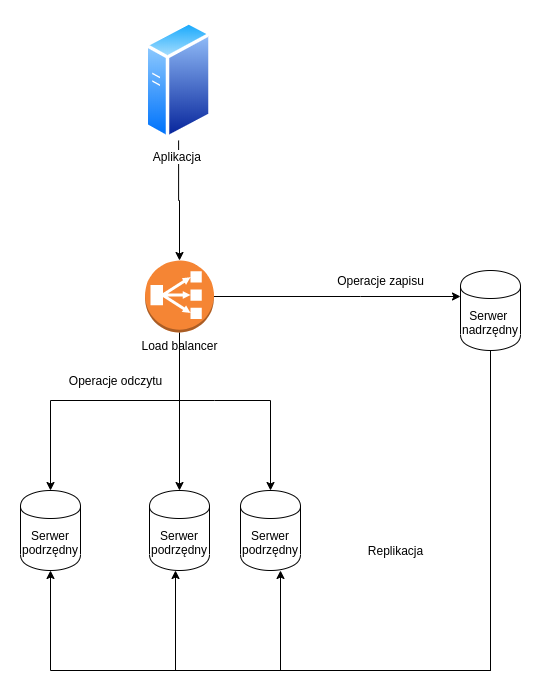
\includegraphics[scale = 0.35]{architektura-z-load-balancerem.png}
	\label{fig:label}
\end{figure}

\subsection{Architektura multi-master}
\textit{Multi-master}, to architektura w której kilka serwerów pełni rolę serwera nadrzędnego (\textit{master}). W takim modelu każdy z serwerów przechowuje pełny zestaw danych oraz może modyfikować je w dowolnym momencie, które następnie są propagowane do pozostałych serwerów. Węzły odpowiadają także za rozwiązywanie potencjalnych konfliktów, które powstały w wyniku równoległych zmian na kilku instancjach. W MySQL realizacją takiej architektury jest replikacją grupową. Replikacja grupowa zapewnia spójność danych pomiędzy serwerami oraz dostepność nawet w przypadku awarii jednego z węzłów. Co istotne, jeżeli jeden z węzłów będzie nieaktywny, klienci z aktywnym połączeniem do tego serwera muszą zostać przełączeni na inny aktywny serwer. Replikacja grupowa nie posiada takiego mechanizmu, dlatego przełączanie ruchu pomiędzy serwerami master powinno być obsłużone na poziomie aplikacji, a najlepiej poprzez umieszczenie \textit{load balancera} pomiędzy aplikacją i serwerami należącymi do grupy.

Wykonanie zmiany w danych na jednym z serwerów, informacja o zmianie przesyłana jest do pozostałych węzłów w postaci plików \textit{binlong}.

Replikacja grupowa jest modelem replikacji optymistycznej. W tym podejściu zakłada się, że wiekszość operacji modyfikacji danych nie będzie powodowała problemów w spójności danych, dlatego nie stosuje się blokad w dostępie do danych, które nie zostały jeszcze zatwierdzone przez wszystkie serwery. Takie założenie może prowadzić do sytuacji, kiedy klient odpytujący dwa różne serwery może otrzymać różne wyniki (brak silnej spójności danych), ale współbieżne modyfikacje są kosztem, który został poniesiony w celu osiągnięcia większej wydajności i skalowalności grupy. W przypadku wystąpienia konfliktów pomiędzy transakcjami, potencjalne konfikty rozwiązywane są po zmodyfikowaniu danych. Z tego powodu ważne jest zachowanie dyscypliny po stronie aplikacji, żeby transakcje operujące na tych samych wierszach w miarę możliwości wykonywane były w ramach pojedynczej transakcji. Istotnym problemem może być wykorzystanie autoinkrementowanych kluczy głównych. Jeżeli dwa lub więcej serwerów będzie przydzielało klucze główne w dokładnie taki sam sposób, doprowadzi to do naruszenia kluczy podstawowych, dlatego bardzo ważne jest uważne ustawienie strategi generowania autoinkrementowanych kluczy podstawowych.

Architektura \textit{multi-master} będzie szczególnie przydatna, kiedy potrzebujemy zapewnić skalowalność operacji zapisu. Dodatkowo realizacja w postaci grupy serwerów zapewnia wygodne skalowanie poprzez elastyczne dodawanie lub odejmowanie węzłów, które zostaną automatycznie dołączone lub odłączone w sposób przeźroczysty dla aplikacji. Jedną z głównych wad realizacji architektury \textit{master-slave} w MySQL jest brak silnej spójności danych, który jednak w zdecydowanej większości sytuacji nie powinien stanowić istotnego problemu. Do wad z pewnością należy zaliczyć również większą złożoność systemu oraz bardziej skomplikowany proces konfiguracji w porównaniu do architektury \textit{master-slave}.


\subsection{Partycjonowanie funkcjonalne}

Funkcje aplikacji można podzielić na pewne podgrupy, które nie łączą się z pozostałymi, na poziomie zapytań SQL. Przykładowo serwis społecznościowy \textit{Facebook} umożliwia odczytywania postów innych użytkoników oraz dokonywanie zakupów w sekcji \textit{Marketplace}. Jeżeli użytkownik przegląda aktualne oferty w dziale \textit{Marketplace}, to zapytania kierowane do bazy danych, będą odpytywać jedynie kilka tabel związanych z zakupami. Jeżeli w tym samym czasie inny użytkownik przegląda posty użytkowników, zapytania nie będą dotyczyć table związanych z zakupami. Oczywiście przykład, który przedstawiłem powyżej, może być rozwiązany za pomocą podziału na osobne serwisy jeszcze na poziomie aplikacji, ale zakładając, że nasza aplikacja nie została podzielona na osobne serwisy i łączy się z jedną bazą danych. W takiej sytuacji obciążenie serwera MySQL jest sumą obciążeń związanych z postami i zakupami. W takim przypadku skutecznym rozwiązaniem jest podział danych pojedynczej aplikacji na zestaw tabel, które nigdy nie są ze sobą łączone. Oczywiście takiego partycjonowania danych nie można przeprowadzać w nieskończoność, ponieważ nie istnieje skończony zbiór tabel, które możemy w taki sposób podzielić. Dodatkowo w ramach każdej z grup jesteśmy ograniczeni możliwościami skalowania pionowego bazy danych. Wadą jest też zwiększona złożoność samej aplikacji, która musi obsłużyć kilka źródeł danych. 

\begin{center}
	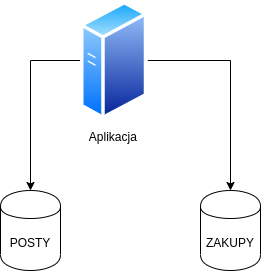
\includegraphics[scale = 0.7]{partycjonowanie-funkcjonalne.png} 
\end{center}


\subsection{Data-sharding}
 
\textit{Data-sharding} wykorzystuje fakt, że rekordy w ramach pojedynczej tabeli są niezależne od siebie. Jako przykład przeanalizowano tabelę \textit{Comments} z testowej bazy \textit{StackOverflow}.
Wiersze w tabeli \textit{Comments} są logicznie powiązane z wierszami w tabeli \textit{Posts}, ale pomiędzy poszczególnymi wierszami w tabeli \textit{Comments} należącymi do innych postów, nie ma relacji. W naszej testowej bazie danych przechowujemy 25 milionów komentarzy. Z obsługą takiej ilości danych, baza danych nie powinna mieć problemów. Niestety z czasem tabela zawierająca komentarze może rozrosnąć się do rozmiarów, których obsłużenie w pojedynczej bazie danych może być problematyczne. Rozwiązaniem tego problemu może być podział pojedynczej tabeli na kilka serwerów. Przykładowo posty wraz z komentarzami o parzystym \textit{PostId} przechowywać na serwerze A, a nieparzyste na serwerze B. Dzięki temu, dwukrotnie zmniejszyliśmy liczbę zapytań do pojedynczej bazy danych, ilość wymaganego miejsca do przechowania postów i komentarzy, rozmiary buforów i indeksów. Wadą takiego rozwiązania jest konieczność obsługi sterowania zapytań do konkretnej bazy na poziomie aplikacji oraz wzrost złożoności logiki aplikacji i systemu bazy danych. Przykładowo chcąc pobrać najnowsze dziesięć postów, musimy wykonać dwa osobne zapytania, pobrać część redundatnych danych i na poziomie aplikacji dokonać wyboru dziesięciu najnowszych postów.


Głownymi przesłankami skłaniającymi do zastosowania tego sposobu skalowalności jest konieczność przechowywania danych w rozmiarach przekraczających możliwości jednego serwera lub skalowanie operacji zapisów, którego nie da się dokonać w ramach replikacji z jednym serwerem nadrzędnym. Sharding danych bardzo dobrze sprawdza się przy jednoczesnym zastosowaniu partycjonowania funkcjonalnego. Przykład zastosowania \textit{data-sharding} wraz z partycjonowaniem funkcjonalnym przedstawiono na poniższym schemacie.

\begin{figure}[!h]
	\centering
	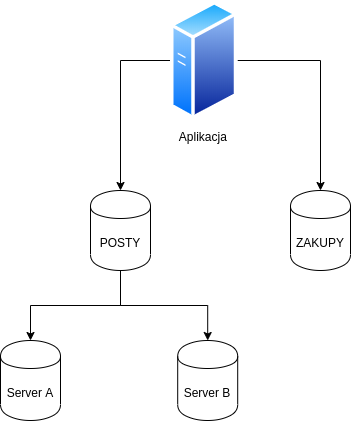
\includegraphics[scale = 0.5]{Partycjonowanie-funkcjonalne-sharding.png}
	\caption{Przykładowa architektura partycjonowania funkcjonalnego}
	\label{fig:label}
\end{figure}


\subsection{InnoDB Cluster}

\begin{figure}[!h]
	\centering
	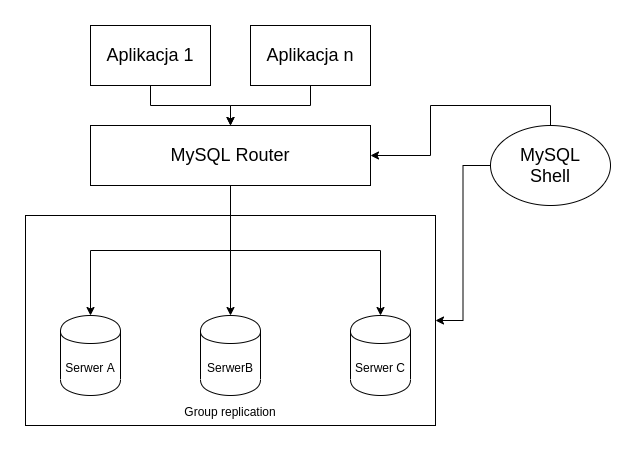
\includegraphics[scale = 0.35]{InnoDb-cluster-architektura.png}
	\caption{Architektura InnoDB Cluster}
	\label{fig:label}
\end{figure}
InnoDb Cluster jest dostępną natywnie kombinacją kilku technologi umożliwiających stworzenie wysoko dostępnej bazy danych w klastrze. Składa się z trzech podstawowych elementów:
\begin{itemize}
	\item \textbf{Group replication} czyli rozwiązania, które zostało opisane w poprzednich rozdziałach (architektura multi-master oraz master-slave).
	\item \textbf{MySQL Shell}, który jest klientem umożliwiającym zarządzanie serwerami MySQL za pomocą jezyków \textit{Java Script}, \textit{Python} lub SQL. Za jego pomocą możemy konfigurować klaster, między innymi poprzez dodawanie lub usuwanie węzłów, tworzenie nowych instancji serwerów, a nawet modyfikowanie danych na poszczególnych serwerach.
	\item \textbf{MySQL Router} będący punktem styku pomiędzy apliakacjami, a instancjami serwerów w klastrze. Router odpowiada za kierowanie ruchem do poszczególnych węzłów jednocześnie uniezależnia klientów od zmian wewnątrz klastra. 
\end{itemize}

Rozwiązanie InnoDB Cluster posiada wszystkie ograniczenia replikacji grupowej przedstawionej w poprzednich sekcjach. Zaletą tego rozwiązania jest wygodniejsza konfiguracja, dzięki możliwości wykorzystania \textit{MySQL shell} w którym możemy administrować naszym klastrem nawet wykorzystując takie języki jak \textit{Java script} czy \textit{Python}. Ważne jest to, że MySQL InnoDB Cluster może działać tylko z tabelami InnoDB, dlatego, żeby użyć klustra należy upewnić się, że wszystkie tabele spełniają ten wymóg.


\subsection{Podsumowanie}
W tym rozdziale przedstawiono kilka architektur możliwych do zrealizowania w MySQL. Przedstawione rozwiązania pokazują, że rozwiązanie wielu zagadnień związanych z optymalizacją może być rozwiązane na poziomie tworzenia architektury bazy danych. Poprzez zastosowanie odpowiedniej architektury możliwe jest zniwelowanie problemów, które występują przy wykorzystaniu pojedyńczego serwera bazy danych. 
//TODO dopisać. Książka strona 271 + link do dokumentacji + przykłady

\section{Indeksy w MySQL}
Indeks jest strukturą danych zwiększającą szybkość operacji wyszukiwania na tabeli. Poprawne stosowanie indeksów jest krytyczne dla zachowania dobrej wydajności bazy danych.
Najprostszą analogią pozwalającą zrozumieć działanie indeksu w bazie danych jest porównanie go z indeksem znajdującym się w książce. Zakładając, że książka nie zawiera indeksu, wyszukiwanie konkretnego słowa lub tematu w najgorszym wypadku wymaga przewertowania całej książki. Z tego powodu w książkach stosuje się indeksy, które zawierają kluczowe słowa użyte w książce. Indeks taki zawiera listę słów oraz stron, na których słowa te występują. Dzięki temu wyszukanie konkretnego słowa wymaga jedynie sprawdzenia numeru strony w indeksie. Jest to szczególnie przydatne przy książkach zawierających dużą liczbę stron. Podobnie jest z tabelami w bazie danych. Przy tabelach o niewielkiej ilości wierszy, wyszukanie konkretnego rekordu trwa krótki nawet przy niestosowaniu indeksów. Indeksy stają się jednak kluczowe wraz ze wzrostem zbioru danych.
W MySQL istnieje wiele rodzajów indeksów, które są implementowane w wartstwie silnika bazy danych, dlatego też nie każdy rodzaj indeksu jest obsługiwany przez wszystkie silniki. W tym rozdziale omówię tylko najpopularniejsze z nich.
\subsection{Indeksy typu B-Tree}
Indeks typu B-Tree jest zdecydowanie najczęściej stosowanym typem indeksu w bazach MySQL i jest domyślnie wybierany przez serwer MySQL podczas tworzenia nowego indeksu. Dlatego właśnie jemu poświęce zdecydowaną wiekszość tego rozdziału.

\paragraph{Struktura}\mbox{}

Indeks typu B-Tree zbudowany jest na bazie struktury B-Drzewa. B-Drzewo jest drzewiastą strukturą danych przechowującą dane wraz z kluczami posortowanymi w pewnej kolejności. Każdy węzeł drzewa może posiadać od M+1 do 2M+1 dzieci, za wyjątkiem korzenia, który od 0 do 2M+1 potomków, gdzie M jest nazywany rzędem drzewa. Dzięki temu maksymalna wysokość drzewa zawierającego n kluczy wynosi $log_M n$. Takie właściwości sprawiają, że operacje wyszukiwania są złożoności asymptotycznej $O(log_M n)$. Chcąc być dokładnym, należy wspomnieć, że MySQL do zapisu indeksów stosuje strukurę B+Drzewa, która jest szczególnym przypadkiem B-Drzewa i zawiera dane jedynie w liściach.
Zastosowanie struktury B+Drzewa sprawia, że liście z danymi znajdują się w jednakowej odległości od korzenia drzewa. Wysoki rząd oznacza niską wysokość drzewa, to z kolei sprawia, że zapytanie wymaga mniejszej ilości operacji odczytu z dysku. Ma to fundamentalne znaczenie, ponieważ dane zapisane są na dyskach twardych, których czasy dostępu są dużo większe niż do pamięci RAM. Dla przykładu, załóżmy, że dana jest tabela zawierająca bilion wierszy, oraz indeks, którego rząd wynosi 64. Operacja wyszukania na danej tabeli wykorzystująca indeks będzie wymagać średnio tylu operacji odczytu, jaka jest wysokość drzewa przechowującego indeksy. Wysokość drzewa obliczamy ze wzoru $\log M n$,gdzie M jest rzędem drzewa równym 64, a n oznacza ilość wierszy. W takim przypadku będziemy potrzebować zaledwie 5 odczytów danych z dysku. Dodatkowo silnik InnoDB nie przechowuje referencji do miejsca w pamięci, w którym znajdują się dane, ale odwołuje się do rekordów poprzez klucz podstawowy, który jednoznacznie identyfikuje każdy wiersz w tabeli.Dzięki temu zmiana fizycznego położenia rekordu nie wymusza aktualizacji indeksu. Indeksy mogą być zakładane zarówno na jedną jak i wiele kolumn. W przypadku indeksu wielokolumnowego, węzły sortowane są w pierwszej kolejności względem pierwszej kolumny indeksu. W następnej kolejności węzły z równymi wartościami pierwszej kolumny, sortowane są względem drugiej itd. Kolejność kolumn jest ustalana na podstawie kolejności podczas polecenia tworzenia indeksu.

\paragraph{Zastosowanie indeksu typu B-Tree}\mbox{}

Aby przedstawić działanie indeksu typu B-Tree na rzeczyczywistym przykładzie przygotowałem dwie tabele. Pierwszą jest tabela \textit{Comments} z bazy danych stackoverflow. Drugą tabelą jest \textit{Init\textunderscore Comments}, która jest kopią tabeli Comments i nie zawiera klucza głównego oraz indeksów.
Dla tabeli \textit{Comments\textunderscore idx} za pomocą polecania \begin{verbatim}
    CREATE INDEX user_post_idx 
ON Comments(UserId,PostId);
\end{verbatim}
utworzyłem indeks typu B-Tree na dwóch kolumnach \textit{first\textunderscore UserId} oraz \textit{last\textunderscore PostId}.

\subparagraph{Dopasowanie pełnego indeksu}\mbox{}

Załóżmy, że w tabeli \textit{Comments} chcemy wyszukać wszystkie komentarze użytkownika o id 1200 do postu o id 910331.

Najpierw wykonamy zapytania na tabeli nie zawierającej indeksów.
 \textit{employees}. 
\begin{verbatim}
    SELECT * FROM Init_Comments WHERE UserId = 1200 AND PostId = 910331;
\end{verbatim}
Zapytanie zwróciło wynik w 13,7 sekundy.

Następnie analogiczne zapytanie wykonałem na tabeli \textit{Comments} zawierającej indeks na obu kolumnach.
\textit{employees\textunderscore idx}. 
\begin{verbatim}
    SELECT * FROM Comments WHERE UserId = 1200 AND PostId = 910331;
\end{verbatim}
Tym razem zapytanie zwróciło wyniki w 0,013 sekundy. Tym razem serwer nie skanował całej tabeli. Z czego wynika różnica w czasie wykonania obu zapytań? Wykorzystując polecenie EXPLAIN dla obu zapytań otrzymujemy ciekawe dane. Rysunek 2 przestawia wynik polecenia EXPLAIN dla pierwszego zapytania, natomiast Rysunek 3 wynik polecania EXPLAIN dla drugiego zapytania. Polecenie EXPLAIN wyjaśnia, że pierwsze zapytania nie będzie korzystać z indeksów, dlatego w kolumnie rows widzimy, że serwer MySQL będzie musiał przeskanować wszystkie 23 miliony wierszy z tabeli \textit{init\textunderscore Comments}. Drguie zapytanie korzysta z indeksu z naszego indeksu. Tym razem serwer będzie musiał przeskanować jedynie 3 wiersze tabeli Comments. 

\begin{figure}[h]
    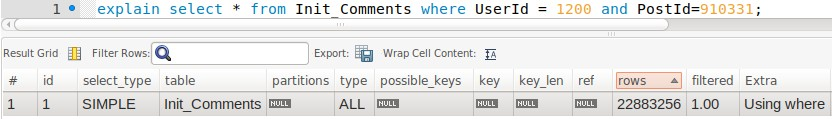
\includegraphics[scale =0.5]{explain1.jpg} 
    \caption{EXPLAIN 1}
\end{figure}

\begin{figure}[h]
    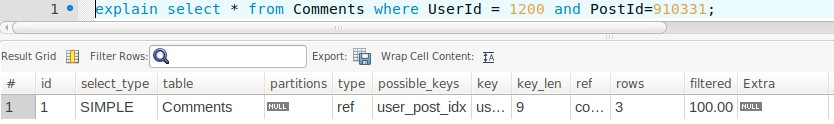
\includegraphics[scale =0.5]{explain2.jpg} 
    \caption{EXPLAIN 2}
\end{figure}

Dopasowanie pełnego indeksu ma miejsce wtedy, kiedy w klauzuli \textit{where} uwzględnimy wszystkie kolumny, na które założony jest indeks. 
\subparagraph{Dopasowanie prefiksu znajdującego się najbardziej na lewo}\mbox{} 
Dopasowanie prefiksu znajdującego się najbardziej na lewo może pomóc w wyszukaniu wsystkich komentarzy użytkownika. Załóżmy, że chcemy znaleźć wszystkie komentarze użytkownika o id 1200.
W tym celu przygotowujemy dwa zapytania. Pierwsze na tabeli \textit{Init\textunderscore Comments}, drugie na tebeli \textit{Comments} zawierającej indeks typu B-Tree, który założyliśmy wcześniej.
\begin{verbatim}
    SELECT * FROM Init_Comments WHERE UserId = 1200;
\end{verbatim}
\begin{verbatim}
    SELECT * FROM Comments WHERE UserId = 1200;
\end{verbatim}
Pierwsze zapytanie zostało wykonane w czasie 12,9 sekundy, natomiast drugie wymagało jedynie 0,0044 sekundy. Ponownie sprawdźmy rezultat polecenia EXPLAIN na obu zapytaniach. W pierwszym zapytaniu serwer po raz kolejny musiał przeszukać wszystkie wiersze w tabeli. Drugie zapytanie wymagało przeszukania 209 wierszy, dlatego że tym razem zapytanie było mniej selektywne niż przy dopasowaniu pełnego indeksu.
\begin{figure}[h]
    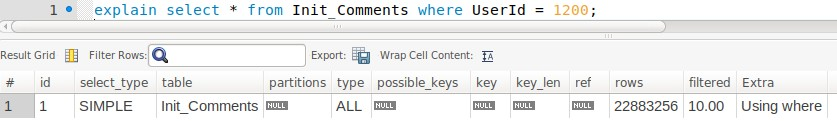
\includegraphics[scale =0.5]{explain3.jpg} 
    \caption{EXPLAIN 3}
\end{figure}

\begin{figure}[h]
    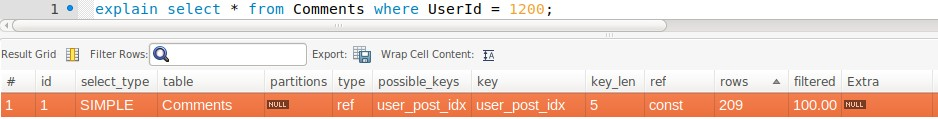
\includegraphics[scale =0.5]{explain4.jpg} 
    \caption{EXPLAIN 4}
\end{figure}

\subparagraph{Dopasowanie zakresu wartości}\mbox{}
Dopasowanie zakresu wartości oznacza wyszukiwanie wartości w danym przedziale. W naszym przypadku może to być wyszukiwanie wszystkich komentarzy użytkowników o identyfikatorach z przedziału od 1990 do 2000.

Ponownie wykonujemy dwa zapytania. Pierwsze na tabeli bez indeksu, drugie na tabeli z indeksem.
\begin{verbatim}
    SELECT * FROM Init_Comments WHERE UserId >1990 AND UserId <2000;
\end{verbatim}

Tym razem pierwsze zapytanie trwało 1.068 sekundy. Drugie zapytanie wykonujemy na tabeli Comments zawierającej indeksy.
\begin{verbatim}
    SELECT * FROM Comments WHERE UserId >1990 AND UserId <2000;
\end{verbatim}
Następnie sprawdzamy wynik polecenia EXPLAIN dla obu zapytań. Przy pierwszym zapytaniu, kolejny raz MySQL przeskanował całą tabelę Init\textunderscore Comments. Drugie natomiast wymagało przeskanowania jedynie wierszy, które zostały zwrócone jako rezultat zapytania.

\begin{figure}[h]
    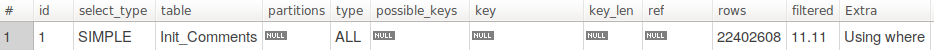
\includegraphics[scale =0.5]{explain5.png} 
    \caption{EXPLAIN 5}
\end{figure}

\begin{figure}[h]
    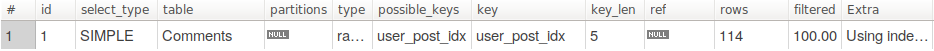
\includegraphics[scale =0.5]{explain6.png} 
    \caption{EXPLAIN 6}
\end{figure}


PREFIX INDEX
będą wymagały przeszukania całej tabeli. Dodatkowo wyszukiwanie za pomocą prefiksu nie będzie optymalne w przypadku indeksu wielokolumnowego dla wszystkich kolumn z wyjątkiem pierwszej. Jest to bezpośrednim następstwem budowy indeksów typu B-Tree i wynika z faktu sortowania kluczy względem pierwszej kolumny.





\subparagraph{Zapytania dotyczące jedynie indeksów}\mbox{}
Zapytania dotyczące jedynie indeksów to zapytania, które wykorzystują jedynie wartości indeksu, a nie do rekordów bazy danych.





 
Indeks jednokolumnowy zawiera klucze posortowane zgodnie z wartościami kolumny, na której założony został indeks. W przypadku indeksów wielokolumnowych węzły sortowane są w kolejności kolumn w indeksie. Zakładając, że indeks został założony na kolumnach k1,k2 oraz k3, dane w pierwszej kolejności zostaną posortowane zgodnie z wartościami kolumny k1. Następnie rekordy z równą wartością kolumny k1 zostaną posortowane zgodnie z wartościami kolumny k2. Analogicznie rekordy z równą wartością kolumny k1 oraz k2 zostaną posortowane zgodnie z wartościami kolumny k3. Zrozumienie tej zasady jest kluczowe do poprawnego korzystania z indeksów typu B-Tree. Taka struktura powoduje, że taki indeks jest użyteczny tylko w przypadku, gdy wyszukiwanie używa znajdujego się najbardziej na lewo prefiksu indeksu.
Kolejnym zastosowaniem indeksu typu B-Tree jest wyszukiwanie na podstawie prefiksu kolumny. Przykładem takiego zapytania może być wyszukiwanie wszystkich pracowników, których nazwiska rozpoczynają się od litery K (zakładamy, że tabela posiada indeks na kolumnie nazwisko). Istotnym jest fakt, że indeks staje się nieprzydany przy wyszukiwaniu na podstawie suffixu lub środkowej wartości. Następnym przypadkiem, w którym indeks typu B-Tree przyśpiesza zapytanie, jest wyszukiwanie na podstawie zakresu wartości. Dla tabeli z indeksem typu B-Tree założonym na kolumnie k, indeks może posłużyć do efektywnego wyszukania wartości z przedziału wartości tej kolumny. Zastosowanie struktury B-Tree powoduje, że sortowanie wyników zapytania względem indeksy jest zdecydowanie bardziej wydajne.


\subsection{Indeksy typu hash}
Indeksy typu hash są dostępne jedynie dla tabel silnika \textit{MEMORY} i są domyślnie ustawianymi indeksami dla takich tabel. Indeksy typu \textit{hash} opierają się na funkcji skrótu liczonej na wartościach indeksowanych kolumn. Dla każdego rekordu takiej tabeli liczona jest krótka sygnatura, na podstawie wartości klucza wiersza. Podczas wyszukiwania wartości na podstawie kolumn indeksowanych tego typu kluczem obliczana jest funkcja skrótu dla klucza, a następnie wyszukuje w indeksie odpowiadających wierwszy. Możliwe jest, że do jednej wartości funkcji skrótu dopasowane zostanie więcej niż jeden różny wiersz. Takie zachowanie wynika bezpośrednio z zasady działania funkcji skrótu, która nie zapewnia unikatowości dla różnych wartości dla zbioru danych wejściowych. Niemniej taka sytuacja nie należy do częstych i nawet wtedy operacja wyszukiwania na podstawie indeksu typu hash jest bardzo wydajna, ponieważ serwer w najgorszym wypadku musi odczytać zaledwie kilka wierszy z tabeli. Stąd wynika największa zaleta indeksów typu \textit{hash} w stosunktu do indeksów \textit{B-Tree}; czas wyszukiwania dowolnego wiersza w tabeli jest stały niezależnie od liczby wierszy. Podstawową wadą indeksu typu hash jest konieczność wyszukiwania na podstawie pełnej wartości klucza. Wynika to z tego, że funkcja skrótu wyliczona na podstawie niepełnego zbioru danych, nie ma korelacji z wartością funkcji wyliczonej na pełnym kluczu. Dodatkowo indeksy hash nie optymalizują operacji sortowania, ponieważ wartości funkcji f1, f2 skrótu dla dwóch rekordów x1 oraz x2, gdzie x1 jest mniejsze od x2 nie zapewniają, że f1 będzie mniejsze od f2. Dodatkowo z racji ograniczonego zbioru wartości funkcji hashującej, mogą występować problemy ze skalowaniem w przypadku dużych zbiorów danych. Po przekroczeniu pewnej liczby wierszy, należy zwiększyć rozmiar klucza indeksu i ponownie obliczyć funkcję dla wszystkich wierszy w tabeli.


\section{Praktyczne problemy}
W tej sekcji zostaną przedstawione przypadki zastosowania teoretycznej wiedzy wraz z praktycznymi przykładami.



\subsection{Sortowanie wyników}
Czasami zdarza się, że chcemy, aby wyniki zapytania były posortowane według pewnej kolejności. Jest to oczywiście pewien dodatkowy nakład, który serwer MySQL musi wykonać podczas wykonania zapytania. W tym podrozdziale pokażę, co zrobić, aby ta operacja nie wypłyneła drastycznie na wydajność naszego zapytania.

Podstawą optymalizacji sortowania jest używanie indeksów typu B-Tree, co wynika bezpośrednio z faktu, że indeks jest posortowany względem jego kolumn. Aby przedstawić działanie indeksów na realnych przykładach przygotowałem do tego bazę StackOverflow. Z bazy usunąłem wszystkie indeksy oraz klucze główne założone na wykorzystywanych w przykładach tabelach, aby nie wpływały one na prezentowane przykłady.

MySQL może użyć indeksu do sortowania wyników w następujących przypadkach.



Najlepszym z możliwych scenariuszy wykorzystania indeksu do sortowania danych jest przypadek, kiedy kolumny użyte do sortowania odpowiadają indeksowi, a kolumny, które chcemy zwrócić jako wynik zapytania są podzbiorem kolumn indeksu.
Weźmy tabelę Users, na którą założymy indeks typu BTREE jak poniżej.

\begin{spverbatim}
	CREATE INDEX Rank_idx ON Users(Reputation, UpVotes);
\end{spverbatim}
Teraz wykonajmy zapytanie:
\begin{spverbatim}
	EXPLAIN SELECT Reputation,UpVotes FROM Users ORDER BY Reputation, UpVotes;
\end{spverbatim}
W takim przypadku poleceni EXPLAIN zwróci w kolumnie EXTRA informację: "Using index", co oznacza, że do sortowania wartości użyty został indeks znajdujący się w kolumnie key, czyli indeks, który przed chwilą stworzyliśmy.

\begin{figure}[H]
	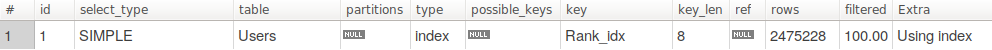
\includegraphics[scale =0.4]{explain15.png} 
\end{figure}
Jeżeli w wyniki chcemy otrzymać jedynie kolumnę \textit{Reputation}, to MySQL wciąż będzie wykorzystywał indeks do sortowania wyników, ponieważ spełnia to warunek zawierania się kolumn rezulatu zapytania w zbiorze kolumn indeksu. Sprawdźmy teraz, co się stanie jeżeli do klauzuli WHERE dodamy kolejną kolumnę:
\begin{spverbatim}
	EXPLAIN SELECT Id, Reputation, UpVotes FROM Users ORDER BY Reputation, UpVotes;
\end{spverbatim}
\begin{figure}[H]
	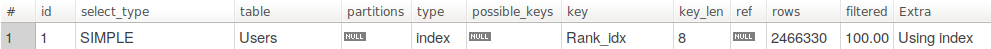
\includegraphics[scale =0.4]{explain16.png} 
\end{figure}
Widzimy, że tym razem MySQL nie wykorzystał indeksu, ale pobrał wszystkie dane i posortował wykorzystując jeden z dostępnych w MySQL algorytmów sortowania. Co ciekawe, nie zawsze musi się tak stać. MySQL na etapie analizy wykonania sprawdza, czy wydajniejsze będzie dla niego sortowanie wyników na podstawie pobranych danych, czy może, jeżeli sortujemy dane względem jednego z indeksów na tabeli, pobrać ten indeks i wykorzystać do wydajniejszego sortowania. Dodajmy teraz klucz główny dla tabeli Users i sprawdźmy, co się stanie jeżeli umieścimy go jako jedną z kolumn wyniku naszego zapytania.
\begin{spverbatim}
	ALTER TABLE Users ADD PRIMARY KEY (Id);
	EXPLAIN SELECT Id, Reputation, UpVotes FROM Users ORDER BY Reputation, UpVotes;
\end{spverbatim}

\begin{figure}[H]
	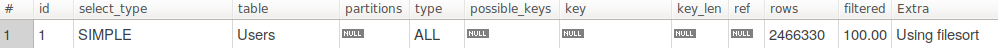
\includegraphics[scale =0.4]{explain17.png} 
\end{figure}
Wynik polecenia EXPLAIN jest interesujący. Przypomnijmy sobie zatem, w jaki sposób MySQL przechowuje dane w indeksie, jeżeli tabela posiada klucz podstawowy. W takim przypadku wiersze w liściach indeksu są identyfikowane za pomocą wartości kluczy głównych. W naszym przypadku wiersze w indeksie są identyfikowane na podstawie kolumny \textit{id}, co oznacza, że indeks zawiera wszystkie kolumny użyte w zapytaniu.

 Kolejnym często używanym zapytaniem jest pobranie wszystkich kolumn z tabeli, ale posortanie ich według określonych kolumn. Weźmy następujące zapytanie:
\begin{spverbatim}
	EXPLAIN SELECT u.* FROM Users u ORDER BY u.UpVotes, u.Reputation;
\end{spverbatim}
Tym razem MySQL znów najprawdopodobniej nie użyje indeksu do posortowania danych. Oczywiście nadal może zdecydować, że efektywniejszym będzie dodatkowe pobranie indeksu i wykorzystanie go do sortowania danych.

Przeanalizujmy teraz następne zapytanie.

\begin{spverbatim}
	EXPLAIN SELECT * FROM Users WHERE Reputation = 1 ORDER BY UpVotes;
\end{spverbatim}
\begin{figure}[H]
	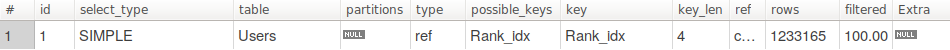
\includegraphics[scale =0.4]{explain18.png} 
\end{figure}
Tym razem MySQL znów wykorzystał indeks, do posortowania wyników. W jaki sposób to zrobił? 
Skorzystał z faktu, że indeksie są posortowane względem kolumn Reputation, a w przypadku, kiedy wartość Reputation jest równa, względem kolumny UpVote, co odpowiada wartości ORDER BY.
Sprawdźmy co się stanie, jeżeli delikatnie zmodyfikujemy zapytanie do postaci:
\begin{spverbatim}
	EXPLAIN SELECT * FROM Users WHERE Reputation > 1000 ORDER BY UpVotes;
\end{spverbatim}

W tym przypadku nie ma jednoznaczej odpowiedzi na pytanie, w jaki sposób MySQL posortuje dane. Optymalizator MySQL musi podjąć decyzję, czy warunki w klauzuli WHERE są wystarczająco selektywne, czy może pobranie indeksu i na jego podstawie przeprowadzenie sortowania będzie efektywniejsze.

\input{ProcedurySkladowane.tex}
\end{document}